\documentclass[mat1]{fmfdelo}
% \documentclass[fin1]{fmfdelo}
% \documentclass[isrm1]{fmfdelo}
% \documentclass[mat2]{fmfdelo}
% \documentclass[fin2]{fmfdelo}
% \documentclass[isrm2]{fmfdelo}

% naslednje ukaze ustrezno napolnite
\avtor{Tom Gornik}
\naslov{Izrek o invarianci odprtih množic}
\title{Domain invariance theorem}

% navedite ime mentorja s polnim nazivom: doc.~dr.~Ime Priimek,
% izr.~prof.~dr.~Ime Priimek, prof.~dr.~Ime Priimek
% uporabite le tisti ukaz/ukaze, ki je/so za vas ustrezni
\mentor{ izr.~prof.~dr.~Jaka Smrekar}
% \mentorica{}
% \somentor{}
% \somentorica{}
% \mentorja{}{}
% \mentorici{}{}

\letnica{2022} % leto diplome

%  V povzetku na kratko opišite vsebinske rezultate dela. Sem ne sodi razlaga organizacije dela --
%  v katerem poglavju/razdelku je kaj, pač pa le opis vsebine.
\povzetek{Zveznost in diskretnost sta v mnogih pogledih povsem nasprotujoča si pojma. Kljub temu se izkaže, da lahko s pomočjo kombinatorike na diskretnih množicah dokažemo veliko lastnosti zveznih funkcij. Glavna prednost takega načina dokazovanja je, da si je postopek dokaza (vsaj v primeru, ko dimenzija ni prevelika) lahko predstavljati in celo skicirati. Pozitivne strani se pokažejo predvsem pri dokazovanju izrekov o obstoju posebnih točk, kot sta negibna točka in ničla funkcije. Primer takega izreka je Poincar\'e-Mirandov izrek, ki je v tem delu dokazan s pomočjo kombinatorike na ogliščih triangulacije kocke in Spernerjeve leme. Dokazano je, da Poincar\'e-Mirandov izrek implicira izrek o invarianci odprtih množic. Na koncu je predstavljena enostavna a pomembna posledica izreka o invarianci odprtih množic, ki jo imenujemo izrek o invarianci dimenzije.
}

%  Prevod slovenskega povzetka v angleščino.
\abstract{Continuity and discreteness are often seen as two opposing concepts, but we can use discrete combinatorics to prove many properties of continuous functions. The main benefit is that we can easily (at least when the dimension is not too large) imagine and also draw some pictures of proof. This works particularly well when we try to prove a theorem on the existence of special points of a function, for example, a fixed point or a zero of a function. One example of this sort of theorem is Poincar\'e-Miranda's theorem which is proved in this work by discrete combinatorics on vertices of a triangulation of a cube and Sperner's lemma. We can show that Poincar\'e-Miranda's theorem implies the domain invariance theorem. In the end, we derive a simple but important corollary, the dimension invariance theorem.  }

% navedite vsaj eno klasifikacijsko oznako --
% dostopne so na www.ams.org/mathscinet/msc/msc2010.html
\klasifikacija{52A20, 54F45, 54H25}
\kljucnebesede{simpleks, Spernerjeva lema, Poincar\'e-Mirandov izrek, izrek o invarianci odprtih množic, izrek o invarianci dimenzij} % navedite nekaj ključnih pojmov, ki nastopajo v delu
\keywords{simplex, Sperner's lemma, Poincar\'e-Miranda's theorem, domain invariance theorem, dimension invariance theorem} % angleški prevod ključnih besed

\zapisiMetaPodatke  % poskrbi za metapodatke in veljaven PDF/A-1b standard

% aktivirajte pakete, ki jih potrebujete
\usepackage{tikz, verbatim, subcaption}
\usepackage{standalone}
\usepackage{import}
\usetikzlibrary{arrows.meta, calc}

\usepackage{bibentry}         % za navajanje literature v programu dela s celim imenom
%\nobibliography{\literatura}
\newcommand{\literatura}{literatura}  % pot do datoteke z literaturo (brez .bib končnice)



% za številske množice uporabite naslednje simbole
\newcommand{\R}{\mathbb R}
\newcommand{\N}{\mathbb N}
\newcommand{\Z}{\mathbb Z}
\newcommand{\C}{\mathbb C}
\newcommand{\Q}{\mathbb Q}


% matematične operatorje deklarirajte kot take, da jih bo Latex pravilno stavil
\DeclareMathOperator{\conv}{conv}
\DeclareMathOperator{\aff}{aff}
\DeclareMathOperator{\diam}{diam}
\DeclareMathOperator{\Int}{Int}
\DeclareMathOperator{\sd}{sd}
\DeclareMathOperator{\dist}{d}


\newcommand{\subdiv}[3] {
\draw ($ 0.5*#2 + 0.5*#3 $) -- #1;
\draw ($ 0.5*#1 + 0.5*#3 $) -- #2;
\draw ($ 0.5*#1 + 0.5*#2 $) -- #3;
}

% vstavite svoje definicije ...
%  \newcommand{}{}
\newcommand{\I}{\mathbb I}
\newcommand{\0}{0}
\newcommand{\pA}{\mathcal A}
\newcommand{\pB}{\mathcal B}
\newcommand{\pU}{\mathcal U}
\newcommand{\pK}{\mathcal K}
\newcommand{\pT}{\mathcal T}

\def\citat#1{,,#1''}


\begin{document}
%####################     1. POGLAVJE: UVOD     ####################
\section{Uvod}
Koncept dimenzije prostora se zdi zelo naraven in intuitiven. V svojih zapisih je o dimenzijah govoril že Aristotel. A ko beremo njegova dela, hitro vidimo, da je bila njegova predstava o dimenzijah drugačna od današnje. Aristotel namreč pravi:~\citat{Premica ima magnitudo v eni smeri, ravnina v dveh smereh, geometrijska telesa pa v treh smereh in poleg teh treh magnitud ni nobene več, kajti te tri so vse}~\cite[str.\ 1, moj prevod]{4dim}. Matematiki so dolgo živeli v prepričanju, da so lahko matematični objekti največ tridimenzionalni. Kasneje so se začele pojavljati potrebe po štiridimenzionalnih objektih, saj so bile na primer v mehaniki enačbe veliko lažje, če je eno dimenzijo predstavljal čas. Tako smo počasi prišli do razmišljanja, da obstajajo večdimenzionalni in celo neskončno dimenzionalni prostori. Problem se pojavi, ko želimo primerjati prostore različnih dimenzij. Intuicija nam pravi, da prostora različnih dimenzij ne moreta biti enaka. V topologiji rečemo, da ne moreta biti homeomorfna. Homeomorfizem je bijektivna zvezna preslikava $f$, katere inverzna preslikava $f^{-1}$ je tudi zvezna. Če lahko prostor $X$ z neko homeomorfno preslikavo preslikamo na prostor $Y$, pravimo, da sta prostora $X$ in $Y$ homeomorfna. Matematiki so že od nekdaj verjeli, da je dimenzija topološka invarianta, kar pomeni, da imata homeomorfna prostora enako dimenzijo. To trditev je bilo zelo težko dokazati ne samo zato, ker je dokaz zapleten, ampak tudi zato, ker ni bilo dobre definicije dimenzije prostora. Kaj sploh je dimenzija prostora? Velikokrat na dimenzijo gledamo kot na najmanjše število parametrov, ki so potrebni za opis nekega prostora. Ta definicija je mnogim matematikom dolgo časa zadoščala, obstajali pa so tudi tisti, ki so vanjo dvomili. Eden prvih, ki je izrazil svoje dvome, je bil nemški matematik Georg Cantor v pismu, ki ga je 5.\ 1.\ 1874 poslal Richardu Dedekindu, prav tako nemškemu matematiku~\cite[str.\ 201]{Gouvea2011}. Čeprav so mnogi matematiki mislili, da je noro poskusiti vsako točko v ravnini izraziti zgolj z enim parametrom s premice, je Cantor to poskušal doseči in leta 1877 je dokazal, da obstaja bijektivna preslikava $c : \R \to \R^n$~\cite[str.\ 203]{Gouvea2011}. To pomeni, da za opis tudi večdimenzionalnih prostorov potrebujemo zgolj en parameter. Kljub presenetljivemu rezultatu pa obstoj take preslikave ni tako zelo ogrožal intuicije, saj je bila preslikava $c$ močno nezvezna. Vedno bolj je postajalo očitno, da je potrebno poiskati dokaz, kar je neuspešno poskusilo kar nekaj matematikov. Potreba po dokazu se je še bolj pokazala, ko je leta 1890 italijanski matematik Giuseppe Peano predstavil krivulje, ki napolnijo cel prostor~\cite{Peano}. To pomeni, da lahko vsako točko v prostoru $\R^n$ zvezno opišemo samo z enim parametrom $t \in \R$. Problem take preslikave je, da ni injektivna, tako da še vedno obstaja upanje, da je intuicija dobra. Potrebno jo je samo posodobiti do trditve, da je dimenzija najmanjše število parametrov, ki jih potrebujemo, da z zvezno injektivno preslikavo opišemo prostor. Ekvivalentno lahko trdimo, da v primeru dveh prostorov $X$ in $Y$, ki sta različnih dimenzij, ne obstaja zvezna bijektivna preslikava $f : X \to Y$. To je prvi dokazal J. L. Brouwer leta 1910~\cite[str.\ 208]{Gouvea2011}. Za dokaz je uporabil nekatere topološke rezultate, npr.\ homotopijo, ki jih mnogi ljubiteljski matematiki in tudi študenti dodiplomskega študija matematike ne poznajo. 

V tem delu bomo predstavili elementaren dokaz tega izreka, ki se izogne abstraktnejšim topološkim trditvam. V poglavju~\ref{raz:simpleksi} bomo razvili potrebno besedišče in spoznali nekaj matematičnih objektov ter njihovih lastnosti, ki so ključni pri dokazih v naslednjih poglavjih. V razdelkih \ref{raz:PM} in \ref{raz:siritev} uporabimo rezultate iz poglavja~\ref{raz:simpleksi} in dokažemo dva ključna gradnika dokaza Brouwerjevega izreka. V poglavju~\ref{raz:ioiom} lahko najdemo dokaz izreka o invarianci odprtih množic in njegove posledice, izreka o invarianci dimenzije. Vrstni red razdelkov je izbran tako, da ohrani nekaj matematične skrivnosti, na koncu pa se vse skupaj sestavi v celoto. Neučakan bralec lahko prebere najprej tudi poglavje~\ref{raz:ioiom} in se kasneje polno motiviran, z vedenjem zakaj in kako je snov uporabna, vrne na začetek ter naknadno zapolni vse vrzeli v dokazu.


%####################     2. POGLAVJE: SIMPLEKSI     ####################
\section{Simpleksi}\label{raz:simpleksi}
V tem razdelku bomo spoznali simplekse in z njimi povezano Spernerjevo lemo. Na koncu bomo nekatere lastnosti simpleksov posplošili tudi na kocke. Poimenovanje za simpleks izvira iz latinske besede \citat{simplex}, ki pomeni preprost oziroma enostaven, saj označuje eno najenostavnejših podmnožic prostora $\R^n$.  Simpleks si lahko predstavljamo kot posplošitev pojma trikotnik, ki je dvodimenzionalen objekt, na ostale dimenzije. Tako v $0$-dimenzionalnem prostoru simpleks označuje točko, enodimenzionalen simpleks predstavlja daljico, v dveh dimenzijah dobimo že znani trikotnik, v treh dimenzijah pa simpleks imenujemo tudi tetraeder. Na sliki~\ref{fig:simplex} so nakazani simpleksi dimenzij $0$, $1$, $2$ in $3$~\cite{simplex}.
%####################   Simpleksi v različnih dimenzijah    ####################
\begin{figure}[h!]  
	\centering
	\import{slike/}{simpleksi.tex}%
	\caption{Nakazani so simpleksi v dimenzijah $0$, $1$, $2$ in $3$.}\label{fig:simplex}
\end{figure}
%###############################################################
Preden podamo natančno definicijo simpleksa, moramo spoznati afino neodvisne množice. Pri tem se bomo držali pravila, da bomo vektor od koordinatnega izhodišča do neke točke $x \in \R^n$ označili z enako oznako kot točko samo, le da bomo nad oznako narisali puščico. Takemu vektorju bomo rekli krajevni vektor točke $x$. Torej, krajevni vektor točke $x \in \R^n$ bomo označili z $\vec{x}$.
\begin{definicija}[\protect{\cite{simplex}}]
Množica točk $x_0, x_1, \dots , x_n \in \R^n$ je \emph{afino neodvisna}, če je množica vektorjev $\vec{x}_1 - \vec{x}_0, \vec{x}_2 - \vec{x}_0, \dots , \vec{x}_n - \vec{x}_0$ linearno neodvisna. V nasprotnem primeru je množica točk \emph{afino odvisna}.
\end{definicija}

Opazimo lahko, da ima v tej definiciji prva točka, tj.\ $x_0$, posebno vlogo. Ker ne govorimo o urejenih množicah in vrstni red elementov ni pomemben, se moramo prepričati, da definicija res karakterizira afino neodvisne množice in ni odvisna od izbire prve točke. Denimo, da je množica vektorjev $\vec{x}_1 - \vec{x}_0, \vec{x}_2 - \vec{x}_0, \dots , \vec{x}_n - \vec{x}_0$ linearno neodvisna. Potem je enakost $\sum\limits_{i=1}^n \alpha_i (\vec{x}_i - \vec{x}_0) = 0$ izpolnjena natanko tedaj, ko so vsi koeficienti enaki $0$, torej velja $\alpha_i = 0$ za vsak $i \in \{ 1, 2, \dots, n \}$. Recimo, da smo za prvi element izbrali neko drugo točko, na primer $x_k$. Radi bi videli, da je potem tudi enakost $\sum\limits_{\substack{i=0 \\ i\neq k}}^n \beta_i (\vec{x}_i - \vec{x}_k) = 0$ izpolnjena samo v primeru, ko so vsi koeficienti v vsoti enaki $0$. V to se prepričamo tako, da uporabimo znan matematični trik ter odštejemo in prištejemo isto vrednost. V tem primeru odštejemo in prištejemo $\vec{x}_0$.
Računamo:
\begin{align*} 
\sum\limits_{\substack{i=0 \\ i \neq k}}^n \beta_i (\vec{x}_i - \vec{x}_k) &=  \sum\limits_{\substack{i=0 \\ i \neq k}}^n \beta_i (\vec{x}_i - \vec{x}_0 + \vec{x}_0 - \vec{x}_k) \\
&=\sum\limits_{\substack{i=0 \\ i\neq k}}^n \beta_i (\vec{x}_i - \vec{x}_0) + \sum\limits_{\substack{i=0 \\ i\neq k}}^n \beta_i (\vec{x}_0 - \vec{x}_k)\\
&= \sum\limits_{i=1}^n \gamma_i (\vec{x}_i - \vec{x}_0),
\end{align*}
kjer koeficiente $\gamma_i$ določimo na naslednji način:
\[  \gamma_i =  \left\{
\begin{array}{cl}\vspace{3pt}
	-\sum\limits_{\substack{i=0 \\ i\neq k}}^n \beta_i &, i = k,\\
	\beta_i &, i \neq k. \\
\end{array} 
\right. \]
Ker je množica vektorjev $\vec{x}_1 - \vec{x}_0, \vec{x}_2 - \vec{x}_0, \dots , \vec{x}_n - \vec{x}_0$ linearno neodvisna, morajo biti koeficienti $\gamma_i = 0$ za vsak $i \in \{1, 2, \dots, n \}$. Torej so tudi koeficienti $\beta_i = 0$ za vsak $i \in \{0, 1, \dots, k-1, k+1, \dots, n \}$. Pokazali smo linearno neodvisnost množice vektorjev $\vec{x}_0 - \vec{x}_k, \vec{x}_1 - \vec{x}_k, \dots , \vec{x}_{k-1} - \vec{x}_k, \vec{x}_{k+1} - \vec{x}_k, \dots, \vec{x}_n - \vec{x}_k$, zato je zgornja definicija dobra. 

S pomočjo točk v prostoru lahko definiramo različne množice. Želeli si bomo take množice, ki imajo naslednjo lastnost.
\begin{definicija}
Množica $K \subset \R^n$ je \emph{konveksna}, če je za vsaki dve točki $x, y \in K$ tudi daljica določena z $x$ in $y$: 
$\left \{ \lambda \vec{x} + (1 - \lambda) \vec{y}; \lambda \in  [0, 1] \right \}$ 
vsa vsebovana v $K$. Primer konveksne množice in primer množice, ki ni konveksna, si lahko pogledamo na sliki~\ref{fig:konveksnost}.
% ####################   Primer in protiprimer konveksne množice    ####################
\begin{figure}[h]  
\centering 
% ####################   Primer konveksne množice    ####################
	\begin{subfigure}[b]{0.4\linewidth} 
	\centering
		\import{slike/}{konveksna.tex}%
		\caption{Množica $A$ je konveksna, saj je vsaka daljica, ki povezuje poljubni točki iz $A$, cela vsebovana v $A$.}\label{fig:konv}
	\end{subfigure}
	\hspace{1cm}
% ####################   Primer nekonveksne množice    ####################
	\begin{subfigure}[b]{0.4\linewidth}
	\centering
		\import{slike/}{nekonveksna.tex}%
		\caption{Množica $B$ ni konveksna, saj del daljice določene s točkama $x$ in $y$, ki je pobarvan rdeče, ni vsebovan v $B$.} \label{fig:nikonv}  
	\end{subfigure}
\caption{Slika prikazuje primer konveksne množice (levo) in množice, ki ni konveksna (desno).}\label{fig:konveksnost} 
\end{figure}
% ######################################################################
\end{definicija}

\begin{definicija}\label{trd:presek-konv}
Presek vseh konveksnih množic, ki vsebujejo množico $A$, imenujemo \emph{konveksna ogrinjača} množice $A$. Konveksno ogrinjačo množice $A$ označimo s $\conv(A)$.
\end{definicija}

Konveksno ogrinjačo točk $x_0, x_1, \dots, x_n$ v prostoru $\R^2$ si lahko predstavljamo kot množico, ki jo omeji elastika, ko jo napnemo čez vse točke in nato spustimo. Prikaz konveksne ogrinjače si lahko pogledamo na sliki~\ref{fig:konvexhull}.
% ####################   Konveksna množica z elastiko    ####################
\begin{figure}[h]  
\centering 
	\import{slike/}{elastika.tex}%
	\caption{Slika prikazuje, kako dobimo konveksno ogrinjačo točk s pomočjo elastike. Na levi strani napnemo elastiko, tako da zaobjame vse točke. Na desni strani pa je prikazano, kako izgleda elastika po tem, ko jo izpustimo in omeji konveksno ogrinjačo (sivo pobarvana množica) prikazanih točk \protect{\cite{convexhull}}.} \label{fig:konvexhull}
\end{figure} 
% #############################################################

\begin{trditev}[\protect{\cite{convexhull}}]
Konveksna ogrinjača množice $A$ je najmanjša konveksna množica, ki vsebuje množico $A$.
%$$A = \left \{ \sum\limits_{i=0}^n \lambda_i \vec{x}_i; \text{ kjer so } \lambda_i \in [0, 1] \text{ za vsak } i \in \{0, 1, \dots, n \} \text{ in } \sum\limits_{i=0}^n \lambda_i = 1  \right \}$$
\end{trditev}
\begin{dokaz}
Jasno je, da je množica $A$ vsebovana v konveksni ogrinjači množice $A$. Prepičati se moramo, da je konveksna ogrinjača konveksna množica. Izberimo poljubni točki, ki pripadata konveksni ogrinjači. Potem ti dve točki pripadata vsaki konveksni množici, ki vsebuje množico $A$. Torej tudi daljica, ki povezuje ti dve točki, leži v vsaki konveksni množici, ki vsebuje množico $A$. Iz tega lahko sklepamo, da daljica, ki povezuje dve poljubni točki, cela leži v konveksni ogrinjači. To pomeni, da je konveksna ogrinjača konveksna množica. Ker je konveksna ogrinjača presek vseh konveksnih množic, ki vsebujejo $A$, je vsebovana v vsaki konveksni množici, ki vsebuje $A$. Zato je najmanjša konveksna množica, ki vsebuje množico $A$.
\end{dokaz}



Iskanje konveksne množice kot preseka vseh konveksnih množic je zamudno. Prav tako je težko preveriti, ali je neka točka vsebovana v konveksni ogrinjači množice $A$. Spodnja trditev nam eksplicitno pove, katere točke so vsebovane v konveksni ogrinjači množice točk $A = \{x_0, x_1, \dots, x_n\}$.
\begin{trditev}[\protect{\cite{convexhull}}]
Konveksna ogrinjača točk $\{x_0, x_1, \dots, x_n\}$ je enaka množici:
$$C =\left \{ \sum\limits_{i=0}^n \lambda_i x_i; \text{ kjer so } \lambda_i \geq 0 \text{ za vsak } i \in \{0, 1, \dots, n \} \text{ in } \sum\limits_{i=0}^n \lambda_i = 1  \right \}.$$
\end{trditev}
Trditev nam pove, da lahko krajevni vektor točke $x \in A = \conv (\{x_0, \dots, x_n\})$ izrazimo kot vsoto $\vec{x} = \sum\limits_{i=0}^n \lambda_i \vec{x}_i$, ki zadošča pogoju $\sum\limits_{i=0}^n \lambda_i = 1$, kjer so vsi koeficienti $\lambda_i$ nenegativna realna števila. Vsoto, ki zadošča zahtevanim pogojem, imenujemo \emph{konveksna kombinacija} točk $x_0, x_1, \dots , x_n$. 

\begin{dokaz}
Najprej se bomo prepričali, da vsaka konveksna množica, ki vsebuje množico $A$, vsebuje vsako konveksno kombinacijo točk iz množice $A$. To bomo dokazali s pomočjo popolne indukcije na število točk, ki nastopajo v konveksni kombinaciji. Če v konveksni kombinaciji nastopata zgolj dve točki, lastnost sledi iz definicije konveksne množice. Denimo, da vsaka konveksna množica, ki vsebuje množico $A$ vsebuje konveksno kombinacijo $m$ točk iz množice $A$. Zapišimo poljubno konveksno kombinacijo $\sum\limits_{i=0}^{m+1} \lambda_i x_i$ $m+1$ točk iz $A$ in se prepričajmo, da je vsebovana v vsaki konveksni množici, ki vsebuje $A$. V primeru, ko je $\lambda_0 = \lambda_1 = \cdots = \lambda_m = 0$, je konveksna kombinacija enaka točki $x_{m+1}$, ki leži v množici $A$. V ostalih primerih zapišemo:

$$\sum\limits_{i=0}^{m+1} \lambda_i x_i =(\lambda_0 + \cdots + \lambda_m) \sum\limits_{i=0}^m \frac{\lambda_i}{\lambda_0 + \cdots + \lambda_m } x_i + \lambda_{m+1} x_{m+1}.$$

Po indukcijski predpostavki točka $\sum\limits_{i=0}^m \frac{\lambda_i}{\lambda_0 + \cdots + \lambda_m } x_i$ pripada vsaki konveksni množici, ki vsebuje $A$. Zato je po definiciji konveksne množice tudi konveksna kombinacija točk $x_0, x_1, \dots, x_{m+1}$ vsebovana v vsaki konveksni množici, ki vsebuje $A$.
Sedaj lahko sklepamo, da je množica $C$ vsebovana v preseku vseh konveksnih množic, ki vsebujejo množico $A$. Ker pa je množica $C$ konveksna, vsebuje presek vseh konveksnih množic, ki vsebujejo množico $A$. Zato je množica $C$ enaka konveksni ogrinjači množice $A$.
\end{dokaz}

Simpleks definiramo kot poseben primer konveksne ogrinjače.
\begin{definicija}[\protect{\cite{convexhull}}]
Naj bo $V = \{x_0, x_1, \dots , x_n \}$ afino neodvisna množica točk v evklidskem prostoru. Konveksni ogrinjači $S$ točk $x_0, x_1, \dots , x_n$ iz množice $V$ pravimo \emph{$n$-dimenzionalni simpleks} ali \emph{$n$-simpleks}. Točke $x_i$ imenujemo \emph{oglišča} simpleksa $S$. Ko želimo poudariti, katera oglišča določajo simpleks, lahko zapišemo tudi $S = \left < x_0, \dots, x_n \right >$. Za vsako neprazno podmnožico $U = \{ y_0, y_1, \dots, y_r \} \subset V$ lahko definiramo simpleks $L = \langle y_0, y_1, \dots, y_r \rangle$, ki ga imenujemo \emph{lice simpleksa} $S$. Če je lice $L$ $(n-1)$-simpleks, ga imenujemo \emph{glavno lice} simpleksa $S$. Unijo vseh glavnih lic simpleksa $S$ imenujemo \emph{rob} simpleksa $S$. Množico točk simpleksa $S$, ki ne ležijo na robu simpleksa, imenujemo \emph{notranjost} simpleksa $S$.
\end{definicija}

Krajevni vektor vsake točke $x \in S = \left < x_0, \dots, x_n \right >$ lahko izrazimo s pomočjo oglišč kot vsoto:
\begin{equation}\label{eqn:tockasimpleksa}
\vec{x} = \sum\limits_{i=0}^n \lambda_i \vec{x}_i,
\end{equation}
ki zadošča pogoju $\sum\limits_{i=0}^n \lambda_i = 1$, kjer so koeficienti $\lambda_i$ nenegativna realna števila. Zakaj smo konveksni ogrinjači dodali pogoj o afini neodvisnosti točk, bomo utemeljili z naslednjim razmislekom. Najprej preoblikujemo izraz~\eqref{eqn:tockasimpleksa}. 
\begin{align*}
\vec{x} &= \sum\limits_{i=0}^n \lambda_i \vec{x}_i \\
&= \sum\limits_{i=0}^n \lambda_i (\vec{x}_i - \vec{x}_0 + \vec{x}_0) \\
&= \sum\limits_{i=0}^n \lambda_i \vec{x}_0 + \sum\limits_{i=1}^n \lambda_i (\vec{x}_i - \vec{x}_0) \\
&= \vec{x}_0 + \sum\limits_{i=1}^n \lambda_i (\vec{x}_i - \vec{x}_0).
\end{align*}
Torej lahko simpleks $S = \langle x_0, x_1, \dots, x_n \rangle$ zapišemo tudi v obliki:
$$S = \vec{x}_0 + \underbrace{\left \{ \sum\limits_{i=1}^n \lambda_i (\vec{x}_i - \vec{x}_0); \lambda_i \geq 0 \text{ za vsak } i \in \{1, \dots, n \} \text{ in } \sum\limits_{i=1}^n \lambda_i \leq 1  \right \}}_{\Delta}.$$
Ker so vektorji $\vec{x}_1 - \vec{x}_0, \vec{x}_2 - \vec{x}_0, \dots, \vec{x}_n - \vec{x}_0$ linearno neodvisni, je množica $\Delta$, ki je določena z njimi, $n$-dimenzionalna podmnožica prostora $\R^n$. Simpleks $S$ je enak množici $\Delta,$ premaknjeni za vektor $\vec{x}_0$, zato je tudi simpleks $S$ $n$-dimenzionalna množica. Če bi bile točke $x_0, x_1, \dots, x_n$ afino odvisne, bi bili vektorji $\vec{x}_1 - \vec{x}_0, \vec{x}_2 - \vec{x}_0, \dots, \vec{x}_n - \vec{x}_0$ linearno odvisni in bi bila množica $\Delta$ največ $(n-1)$-dimenzionalna. Tako z vsakim dodatnim ogliščem povečamo dimenzijo simpleksa.
Števila $\lambda_i$ v enačbi~\eqref{eqn:tockasimpleksa} so \emph{baricentrične koordinate} točke $x$, kar zapišemo kot $x = (\lambda_0, \dots, \lambda_n)_b$. Koordinate vektorja $\vec{x}$ so zvezne funkcije točke $x$, zato so tudi baricentrične koordinate točke $x$ zvezno odvisne od položaja točke $x$. Preden nadaljujemo, se moramo prepričati, da so baricentrične koordinate dobro definirane.
\begin{trditev}\label{trd:zveznost-baricentra}
Baricentrične koordinate točke $x \in \left <x_0, \dots, x_n \right >$ so enolično določene.
\end{trditev}
\begin{dokaz}
Recimo, da $x$ izrazimo na dva načina kot $x = \left (\alpha_0, \dots, \alpha_n \right )_b = \left (\beta_0, \dots, \beta_n \right )_b$. Potem lahko zapišemo 
$$\sum_{i=0}^n \alpha_i \vec{x}_i = \sum_{i=0}^n \beta_i \vec{x}_i.$$
Če enačbi odštejemo desno stran, dobimo 
$$\sum_{i=0}^n \alpha_i \vec{x}_i - \sum_{i=0}^n \beta_i \vec{x}_i = 0,$$
kar preoblikujemo v enačbo
$$\sum_{i=0}^n (\alpha_i - \beta_i) \vec{x}_i  = 0.$$
Uporabimo že znan trik ter odštejemo in prištejemo isto vrednost,
$$\sum_{i=0}^n (\alpha_i  - \beta_i) \cdot (\vec{x}_i - \vec{x}_0 + \vec{x}_0) = 0.$$
Enačbo lahko zapišemo z dvema vsotama
$$\sum_{i=1}^n (\alpha_i  - \beta_i) \cdot (\vec{x}_i -\vec{x}_0) + \sum_{i=0}^n (\alpha_i  - \beta_i) \cdot \vec{x}_0= 0,$$
kjer pri prvi vsoti parameter $i$ začne teči pri $1$, saj je pri vrednosti $0$ tudi vrednost sumanda  $(\alpha_0 - \beta_0) \cdot (\vec{x}_0 -\vec{x}_0)$ enaka $0$. Druga vsota je enaka $0$, saj velja:
$$\sum_{i=0}^n (\alpha_i  - \beta_i) \cdot \vec{x}_0= \vec{x}_0 \left (\sum_{i=0}^n \alpha_i  - \sum_{i=0}^n \beta_i \right) = \vec{x}_0 (1 - 1)= 0.$$
Tako pridemo do enačbe 
$$\sum_{i=1}^n (\alpha_i  - \beta_i) \cdot (\vec{x}_i - \vec{x}_0)=0.$$
Ker je množica vektorjev $\{ \vec{x}_i - \vec{x}_0 \in \R^n; i = 1, 2, \dots, n\}$ linearno neodvisna, morajo biti koeficienti $\alpha_i  - \beta_i $ enaki $0$ za vsak $i = 1, 2, \dots, n$. Zato velja $\alpha_i  = \beta_i$ za vsak $i \in \{ 1, \dots, n \}$. Sedaj lahko iz enakosti
$$\sum_{i=0}^n \alpha_i  = \sum_{i=0}^n \beta_i $$
in iz dejstva, da je koeficient $\alpha_i$ enak koeficientu $\beta_i$ za vsak $i = 1, \dots, n$, sklepamo, da sta enaka tudi koeficienta $\alpha_0$ in $\beta_0$.
\end{dokaz}

Pri dokazovanju različnih rezultatov s pomočjo simpleksov si večkrat pomagamo z delitvijo simpleksa na manjše simplekse. Da imamo čim več nadzora pri dokazovanju, si pomagamo s pojmom simplicialnega kompleksa.
\begin{definicija}%\label% ##########  simplicialni kompleks  #################
Množica simpleksov $\pK$ v evklidskem prostoru je \emph{simplicialni kompleks}, če zadošča naslednjima pogojema:
\begin{enumerate}\label{simpl-kompleks}
\item Vsako lice $L$ vsakega simpleksa $S \in \pK$ je tudi vsebovano v $\pK$.\label{simpl-kompleks1}
\item Neprazen presek dveh simpleksov iz $\pK$ je lice obeh simpleksov.\label{simpl-kompleks2}
\end{enumerate}
Unijo vseh simpleksov iz simplicialnega kompleksa $\pK$ bomo označili s $| \pK |$.
\end{definicija}
Iz simpleksa lahko konstruiramo simplicialni kompleks in na ta način dobimo posebno delitev simpleksa.
\begin{definicija}
Simplicialni kompleks $\pT$ je \emph{triangulacija} simpleksa $S$, če je $|\pT| = S$.
\end{definicija}

% ####################   Primer in protiprimer triangulacije    ####################
\begin{figure}[h]  
\centering 
% ####################   Primer triangulacije    ####################
	\begin{subfigure}[b]{0.4\linewidth} 
	\centering
		\import{slike/}{triang.tex}%
		\caption{Delitev je triangulacija.} \label{fig:triang}
	\end{subfigure}
	\hspace{1cm}
% ####################   Primer delitve, ki ni triangulacija    ####################
	\begin{subfigure}[b]{0.4\linewidth}
	\centering
		\import{slike/}{nitriang.tex}%
		\caption{Delitev ni triangulacija.} \label{fig:nitriang}  
	\end{subfigure}
\caption{Slika prikazuje primer triangulacije (levo) in primer delitve, ki ni triangulacija (desno), saj presek osenčenih simpleksov ni lice obeh simpleksov.}
\end{figure} 
% ##################################################################
Pri poljubnih delitvah simpleksa $S$ nimamo nadzora nad tem, kako veliki simpleksi nastopajo v delitvi. Želeli bi si poiskati take delitve, ki vsebujejo zgolj simplekse, ki so manjši od vnaprej predpisane vrednosti $\varepsilon > 0$.
Za mero, kako velik je simpleks, imamo več možnosti. Izbrali bomo diameter, ki ga definiramo na naslednji način.
\begin{definicija}
Največjo razdaljo med dvema točkama simpleksa $S$ imenujemo \emph{diameter} simpleksa $S$. Torej,
$$\diam(S) = \max \{ \dist(x, y); x, y \in S\}.$$
\end{definicija}

Simpleks $S$ je kompaktna množica. Zvezna funkcija definirana na kompaktni množici zavzame maksimum, zato je diameter simpleksa $S$ dobro definiran.
Sedaj, ko imamo mero za velikost simpleksa, si poglejmo, kako lahko celoten prostor $\R^n$ razdelimo na enako velike simplekse. Izberimo naravno število $k$ in pozitivno realno število $a$. Definiramo bazo $\pB$ prostora $\R^n$ z baznimi vektorji $\vec{e}_i := (0, \dots, 0, \frac{a}{k}, 0, \dots, 0)$, pri katerih je edina neničelna koordinata na $i$-tem mestu enaka $\frac{a}{k}$. Definiramo množico $Z_k := \left\{ j \cdot \frac{a}{k}; j \in \Z \right\}$ in označimo z $Z_k^n$ kartezični produkt $n$ kopij množice $Z_k$. Naj bo $P(n)$ množica permutacij množice $\{1, \dots, n \}$.
Množica, ki vsebuje vse simplekse $S = \langle z_0, z_1, \dots, z_n \rangle$, ki zadoščajo pogojema:
\begin{itemize}
\item Množica točk $\{ z_0, z_1, \dots, z_n \}$ je podmnožica množice $Z_k^n$ in
\item obstaja taka permutacija $\pi \in P(n)$, da je 
\begin{equation*}
z_1 = z_0 + \vec{e}_{\pi(1)}, z_2 = z_1 + \vec{e}_{\pi(2)}, \dots, z_n = z_{n-1} + \vec{e}_{\pi(n)},
\end{equation*}
\end{itemize}
razdeli prostor $\R^n$ na $n$-dimenzionalne simplekse.
%se imenuje \emph{$k$-ta mrežna delitev} prostora $\R^n$. 
Če množici dodamo še vsa lica simpleksov iz te množice, dobimo $k$-to mrežno delitev prostora $\R^n$, ki jo označimo z $M_{\frac{a}{k}}^n$.
Prepričajmo se, da množica $M_{\frac{a}{k}}^n$ zadošča pogojema definicije \ref{simpl-kompleks}. Hitro vidimo, da izpolnjuje pogoj \eqref{simpl-kompleks1}. Preveriti moramo še, da je neprazen presek dveh simpleksov iz $M_{\frac{a}{k}}^n$ lice obeh simpleksov. Ker je vsak simpleks iz $M_{\frac{a}{k}}^n$ lice nekega $n$-simpleksa iz $M_{\frac{a}{k}}^n$, je dovolj, če pokažemo, da je neprazen presek dveh $n$-simpleksov iz množice $M_{\frac{a}{k}}^n$ lice obeh simpleksov. Vsak $n$-simpleks $S = \langle z_0, \dots, z_n \rangle \in  M_{\frac{a}{k}}^n$ je natančno določen s točko $z_0 = (z_{0,1}, z_{0, 2}, \dots, z_{0,n})$ in permutacijo $\pi \in P(n)$. Če poznamo ta dva podatka, lahko $n$-simpleks $S$ zapišemo tudi kot množico vseh točk $t=(t_1, \dots, t_n)$, ki zadoščajo pogojem:
$$\frac{a}{k} \geq t_{\pi(1)} - z_{0, \pi(1)}  \geq t_{\pi(2)} - z_{0, \pi(2)} \geq \cdots \geq t_{\pi(n)} - z_{0, \pi(n)} \geq 0.$$
%####################    Slika definicije soseda ####################
\begin{figure}[h!]    
	\centering
		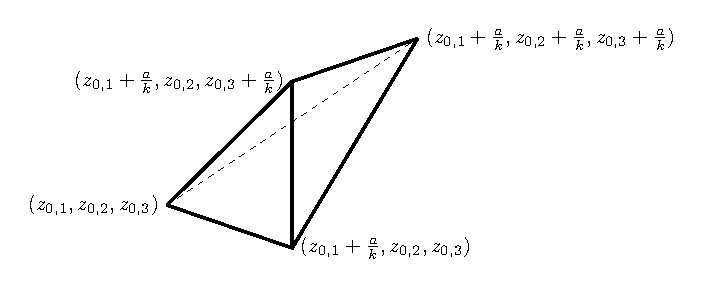
\includegraphics[width=0.8\textwidth]{slike/meje.pdf}
	\caption{Slika prikazuje primer simpleksa, ki je določen z začetno točko $z_0$ in permutacijo $\pi = (2 3)$.}
\end{figure}
%#######################################################
Izberimo poljubni naravni števili $i$ in $j$. Brez izgube splošnosti lahko predpostavimo, da je $\pi(i) < \pi(j)$. Oglišča simpleksa so dobljena tako, da vedno povečamo eno koordinato, zato imajo $\pi(i)$-to koordinato večjo ali enako od $\pi(j)$-te koordinate. Ker simpleks dobimo kot afino kombinacijo oglišč, imajo tudi vse točke simpleksa $\pi(i)$-to koordinato večjo ali enako od $\pi(j)$-te koordinate.
Za vsak par naravnih števil $1 \leq i, j \leq n$ lahko iz zgornjih pogojev razberemo neenakost $t_i - z_{0, i}  \geq t_j - z_{0, j}$ ali $t_i - z_{0, i}  \leq t_j - z_{0, j}$, ki nam pove, v katerem polprostoru, omejenem s hiperravnino $t_i - z_{0, i} = t_j - z_{0, j}$, leži $n$-simpleks $S$.
Lica $n$-simpleksa $S$ dobimo tako, da nekaj neenačajev spremenimo v enačaj. Naj bo $S \in M_{\frac{a}{k}}^n$ $n$-simpleks, ki zadošča pogojem
\begin{equation}\label{eq:pogojiS}
\frac{a}{k} \geq t_{\pi(1)} - z_{0, \pi(1)}  \geq t_{\pi(2)} - z_{0, \pi(2)} \geq \cdots \geq t_{\pi(n)} - z_{0, \pi(n)} \geq 0
\end{equation}
in naj bo $R \in M_{\frac{a}{k}}^n$ $n$-simpleks, ki zadošča pogojem
\begin{equation}\label{eq:pogojiR}
\frac{a}{k} \geq t_{\rho(1)} - w_{0, \rho(1)}  \geq t_{\rho(2)} - w_{0, \rho(2)} \geq \cdots \geq t_{\rho(n)} - w_{0, \rho(n)} \geq 0.
\end{equation}
%Če za vsako naravno število $l \leq n$ velja enakost $z_{0, \pi(l)} = w_{0, \rho(l)}$, je presek simpleksov $S$ in $R$ neprazen. Iz pogojev \eqref{eq:pogojiS} in \eqref{eq:pogojiR} lahko za vsak par naravnih števil $1 \leq i, j \leq n$ ugovovimo, v katerem polprostoru omejenem s hiperravnino $t_i - z_{0, i} = t_j - z_{0, j}$ ležita simpleksa $S$ in $R$. Kadar ležita v istem polprostoru, tudi presek leži v tem podprostoru. Če pa ležita v različnih polprostorih, leži presek $S \cap R$ na hiperravnini $t_i - z_{0, i} = t_j - z_{0, j}$, zato moramo pri pogojih \eqref{eq:pogojiS} in \eqref{eq:pogojiR} ustrezno neenakost spremeniti v enakost. Ko postopek naredimo za vsak par naravnih števil $1 \leq i, j \leq n$, dobimo presek simpleksov $S$ in $R$ kot lice obeh simpleksov.

Če točki $z_0$ in $w_0$ ležita na istem simpleksu iz $M_{\frac{a}{k}}^n$, za vsako naravno število $l \leq n$ velja neenakost $|z_{0, \pi(l)} - w_{0, \rho(l)}| \leq \frac{a}{k}$. Tedaj lahko pogoje, katerim zadoščajo točke preseka $S \cap R = L$, zapišemo na naslednji način. Naj bo $E \subset \{1, 2, \dots, n \}$ množica tistih naravnih števil $e$, za katera je $z_{0,e} = w_{0, e}$. Za vsako naravno število $l \in \{1, 2, \dots, n \} \setminus E$ pri pogojih \eqref{eq:pogojiS} in \eqref{eq:pogojiR} spremenimo neenačbo $\frac{a}{k} \geq t_l - \min(z_{0, l}, w_{0, l})$ v enačbo $\frac{a}{k} = t_l - \min(z_l, w_l)$ in neenačbo $t_l - \max \{z_l, w_l \} \geq 0$ v enačbo $t_l - \max \{z_l, w_l \} = 0$. 
Iz pogojev \eqref{eq:pogojiS} in \eqref{eq:pogojiR} lahko za vsak par naravnih števil $i, j \in E$ ugotovimo, v katerem polprostoru, omejenem s hiperravnino $t_i - z_{0, i} = t_j - z_{0, j}$ ležita $n$-simpleksa $S$ in $R$. Kadar ležita v istem polprostoru, tudi presek $L$ leži v tem podprostoru, zato presek $L$ zadošča isti neenakosti. Če pa $n$-simpleksa $S$ in $R$ ležita v različnih polprostorih, leži presek $L$ na hiperravnini $t_i - z_{0, i} = t_j - z_{0, j}$, zato moramo pri pogojih \eqref{eq:pogojiS} in \eqref{eq:pogojiR} ustrezno neenakost spremeniti v enakost. Ugotovimo, da presek $L$ ustreza enakim pogojem kot simpleksa $S$ in $R$, le da smo nekaj neenačajev spremenili v enačaje, zato je presek $L$ lice simpleksov $S$ in $R$.
%Iz pogojev \eqref{eq:pogojiS} in \eqref{eq:pogojiR} lahko za vsak par naravnih števil $1 \leq i, j \leq n$ razberemo katerim neenakostim zadoščata koordinati $x_i$ in $x_j$. Če velja 
%v katerem polprostoru omejenem s hiperravnino $t_i - z_{0, i} = t_j - z_{0, j}$ ležita simpleksa $S$ in $R$. Kadar ležita v istem polprostoru, tudi presek leži v tem podprostoru. Če pa ležita v različnih polprostorih, leži presek $S \cap R$ na hiperravnini $t_i - z_{0, i} = t_j - z_{0, j}$, zato moramo pri pogojih \eqref{eq:pogojiS} in \eqref{eq:pogojiR} ustrezno neenakost spremeniti v enakost. Ko postopek naredimo za vsak par naravnih števil $1 \leq i, j \leq n$, dobimo presek simpleksov $S$ in $R$ kot lice obeh simpleksov.
Če obstaja tako naravno število $l \leq n$, da je $|z_{0, l} - w_{0, l}| \geq \frac{2a}{k}$, je presek simpleksov $S$ in $R$ prazen.

Pokazali smo, da sta poljubna simpleksa ali disjunktna ali pa si delita lice. V naslednji trditvi bomo pokazali, da sta simpleksa $S$ in $R$ edina $n$-simpleksa, ki vsebujeta $(n-1)$-simpleks $L$, če je presek $L$ $n$-simpleksov $S$ in $R$ glavno lice obeh simpleksov.
\begin{trditev}
Če je $S = \langle z_0, z_1, \dots, z_n \rangle$ simpleks iz $k$-te mrežne delitve prostora $\R^n$, potem za vsako oglišče $z_i$ simpleksa $S$ obstaja natanko en tak simpleks $T = S[i]$ iz $k$-te mrežne delitve, da je 
$$S \cap T = \langle z_0, \dots, z_{i-1}, z_{i+1}, \dots, z_n \rangle.$$
\end{trditev}

\begin{dokaz}
Vemo, da obstaja taka permutacija $\pi \in P(n)$, da za oglišča simpleksa $S = \langle z_0, z_1, \dots, z_n \rangle$ veljajo naslednje enakosti:
\begin{equation}\label{eq:orientiran-simpleks}
z_1 = z_0 + \vec{e}_{\pi(1)}, z_2 = z_1 + \vec{e}_{\pi(2)}, \dots, z_n = z_{n-1} + \vec{e}_{\pi(n)}.
\end{equation}
Naj bo $i$-ti sosed $S[i]$ simpleksa $S$ definiran na naslednji način:
\begin{enumerate}
\item Če je $0 < i < n$,  je $S[i] = \langle z_0, \dots, z_{i-1}, w_i, z_{i+1}, \dots, z_n \rangle$, kjer je $w_i = z_{i-1} + (z_{i+1} - z_i) = z_{i-1} + \vec{e}_{\pi(i+1)}$.
\item Če je $i = 0$, je $S[i] = \langle z_1, \dots, z_n, w_0 \rangle$, kjer je $w_0 = z_n + (z_1 - z_0) = z_{n} + \vec{e}_{\pi(1)}$.
\item Če je $i = n$, je $S[i] = \langle w_n, z_0, \dots, z_{n-1} \rangle$, kjer je $w_n = z_0 + (z_{n-1} - z_n) = z_{0} - \vec{e}_{\pi(n)}$.
\end{enumerate}
%####################    Slika definicije soseda ####################
\begin{figure}[h!]    
	\centering
		\import{slike/}{sosed}
	\caption{Na sliki vidimo del mrežne delitve prostora $\R^2$ in prikaz sosedov simpleksa $S$.}
\end{figure}
%#######################################################
Prepričajmo se, da je definicija $i$-tega soseda dobra.

%$$S \cap S[i] = \langle z_0, \dots, z_{i-1}, z_{i+1}, \dots, z_n \rangle.$$###############################################

Pokazati moramo, da je simpleks $S[i]$ vsebovan v $k$-ti mrežni delitvi prostora $\R^n$ za vsak $i = 0, \dots, n$. Hitro lahko vidimo, da so za vsako število $i = 0, \dots, n$ oglišča simpleksa $S[i]$ vsebovana v množici $Z_k^n$. Poiščimo permutacijo, s pomočjo katere lahko oglišča simpleksa $S[i]$ zapišemo kot v enačbi \eqref{eq:orientiran-simpleks}. 
Definirajmo permutacijo $\tau(i) \in P(n)$:
\begin{enumerate}
\item Če je $0 < i < n$, je permutacija $\tau$ transpozicija, ki med seboj zamenja $i$-ti in $(i+1)$ element, ostale pa pusti pri miru.
\item Če je $i = 0$, je permutacija $\tau$ cikel, ki vse elemente premakne za eno mesto nazaj, prvi element pa postavi na konec.
\item Če je $i = 0$, je permutacija $\tau$ cikel, ki vse elemente premakne za eno mesto naprej, zadnji element pa postavi na začetek.
\end{enumerate}
Iskana permutacija je potem $\rho = \pi \circ \tau$.
Prepričajmo se, da je $S[i]$ edina izbira za ustreznega soseda. Brez izgube splošnosti lahko predpostavimo, da je $z_0 = 0$. Opazimo, da enačba \eqref{eq:orientiran-simpleks} za simpleks $S \in M_{\frac{a}{k}}^n$ podaja končno zaporedje točk z začetnim členom $(0, \dots, 0)$ in končnim členom $(\frac{a}{k}, \dots, \frac{a}{k})$. Vsak naslednji člen dobimo iz predhodnega tako, da eno koordinato povečamo za $1$. V našem primeru to pomeni, da eno koordinato spremenimo iz $0$ v $\frac{a}{k}$. Katero koordinato spremenimo, določa predpis \eqref{eq:orientiran-simpleks}. To zaporedje je urejeno, saj se koordinate povečujejo, člena pa sta lahko sosednja, kadar se razlikujeta v eni sami koordinati. Če odstranimo začetno točko tega zaporedja, dobimo zaporedje z $n-1$ členi. Dopolnimo ga lahko samo na dva načina. Člen, ki smo ga odvzeli, lahko dodamo na začetek ali pa dodamo člen na konec zaporedja tako, da zadnjemu členu povečamo koordinato, ki se v krajšem zaporedju nikoli ne spremeni. V prvem primeru zaporedje ustreza simpleksu $S$, v drugem pa simpleksu $S[0]$. Člena ne moremo vriniti v sredino krajšega zaporedja, saj se potem sosednji členi ne bi razlikovali v natanko eni koordinati. 
Podobno lahko postopamo v primeru, ko odvzamemo zadnji element zaporedja. Recimo, da smo odvzeli $i$-ti člen zaporedja. Potem se $(i-1)$-i člen in $(i+1)$-i člen razlikujeta v dveh koordinatah. Označimo ti dve koordinati s $p$ in $r$. Da dopolnimo zaporedje, moramo dodati en člen na $i$-to mesto. To lahko storimo tako, da dodamo člen, ki se v vseh koordinatah ujema z $(i+1)$-im členom, le na $p$-ti ali na $r$-ti koordinati se ujema z  $(i-1)$-im členom. V enem primeru dobimo zaporedje, s katerim smo začeli, v drugem pa zaporedje, ki ustreza simpleksu $S[i]$.
Simpleks $S[i]$ ustreza lastnosti:
$$S \cap S[i] = \langle z_0, \dots, z_{i-1}, z_{i+1}, \dots, z_n \rangle$$
in je edini simpleks s to lastnostjo.
\end{dokaz}

%pot $P$ po točkah $z_0, z_1, \dots, z_n$. S potjo $P$ mislimo na točke $z_0, z_1, \dots, z_n$ in na $1$-dimenzionalna lica simpleksa $S$, ki jih povezujejo. Vsako $1$-dimenzionalno lice iz poti bomo imenovali korak. Koraki so narejeni v smeri vektorjev $\vec{e}_i$ za $i = 1, \dots, n$. Če pogledamo pot samo na licu $L = \langle z_0, \dots, z_{i-1}, z_{i+1}, \dots, z_n \rangle$ imamo dve možnosti.Pot na licu $L$ je lahko za en korak krajša od poti $P$. V tem primeru lahko pot s korakom podaljšamo na začetku ali na koncu. V enem primeru dobimo simpleks $S$, v drugem pa soseda $S[i]$. To dokaže trditev v primeru, ko je $i \in \{0, n\}$. Druga možnost je, da je pot na licu za dva koraka krajša od poti $P$. V Tem primeru imamo dve povezani poti. Povežemo ju lahko na istem mestu, kjer ju poveže pot $P$. V nasprotnem primeru dobimo cikel sestavljen iz baznih vektorjev, kar pa ni mogoče. Torej lahko pot povežemo na dva načina, saj imamo dva različno usmerjena koraka, ki ju lahko uporabimo v dveh različnih vrstnih redih. V enem primeru dobimo simpleks $S$, v drugem pa njegovega soseda $S[i]$. Torej je sosed res enolično določen.
S pomočjo delitve prostora lahko definiramo triangulacijo simpleksov. Definiramo $k$-to mrežno triangulacijo simpleksa $S = \langle x_0, x_1, \dots, x_n \rangle \in M^n_{\frac{a}{1}}$ kot simplicialni kompleks, ki vsebuje vse simplekse iz mrežne delitve $M^n_{\frac{a}{k}}$ prostora $\R^n$, ki so vsebovani v simpleksu $S$.
Naj bo $R = \langle y_0, y_1, \dots, y_n \rangle$ poljuben $n$-simpleks v prostoru $\R^n$. Definirajmo homeomorfizem $h : S \to R$ s predpisom
$$h \left( \sum_{i=0}^n t_i x_i \right) = \sum_{i=0}^n t_i y_i,$$
kjer za vsak $i=0, 1, \dots, n$ realna števila $t_i$ zadoščajo pogojem $t_i \geq 0$ in $\sum_{i=0}^n t_i = 1$.
S preslikavo $h$ prenesemo triangulacijo simpleksa $S$ na simpleks $R$. Taki triangulaciji rečemo \emph{$k$-ta mrežna delitev} simpleksa $R$. Za oznako $k$-te mrežne delitve $n$-simpleksa bomo uporabljali kar $M_k^n$, saj število $a$ na to delitev nima vpliva. 

Radi bi videli, da se s povečevanjem števila $k$ simpleksi v $k$-ti mrežni delitvi zmanjšujejo.
Pokažimo, da je diameter simpleksa $S = \langle v_0, v_1, \dots v_n \rangle$ enak dolžini najdaljše stranice. Izračunamo razdaljo med točkama $x, y \in S$:
$$\dist(x, y) = \| \vec{x} - \vec{y} \|.$$
Krajevni vektor točke $y$ lahko zapišemo s pomočjo oglišč simpleksa:
$$\left\| \vec{x} - \sum_{i=0}^n t_i \vec{v}_i \right\|,$$
kar lahko preoblikujemo in ocenimo:
$$\left \| \sum_{i=0}^n t_i (\vec{x} - \vec{v}_i)\right \| \leq \sum_{i=0}^n t_i \| (\vec{x} - \vec{v}_i) \| \leq \sum_{i=0}^n t_i \max_{j=0, \dots, n}(\| (\vec{x} - \vec{v}_j) \|) = \max_{j=0, \dots, n}(\| (\vec{x} - \vec{v}_j) \|).$$
Ugotovili smo, da je razdalja največja, ko je $y$ oglišče simpleksa $S$. Zaradi simetričnosti razdalje mora biti za maksimizacijo razdalje tudi $x$ oglišče simpleksa.
Ker so dolžine stranic simpleksa $R$ iz $k$-te mrežne delitve simpleksa $S$ za faktor $k$ manjše od stranic simpleksa $S$, velja $\diam(R) = \frac{1}{k} \cdot \diam(S)$.

Pri obravnavi triangulacij simpleksov lahko počnemo veliko stvari. Ena taka, ki bi se jo lahko spomnil celo otrok v vrtcu, je, da bi simplekse iz triangulacije pobarvali. Tako lahko dobimo zanimive slike. Mi bomo obravnavali lastnosti, ki jih opazimo pri barvanju oglišč določene triangulacije.
\begin{definicija}[\protect{\cite[str.\ 9, definicija 1]{Ahlbach}}]
Naj bo podan $n$-simpleks $S \in \R^n$ s triangulacijo $\pT$. Označimo množico oglišč triangulacije $\pT$ z $V$. Preslikavo $b : V \to \left \{0, 1, \dots, n \right \} $ imenujemo \emph{barvanje triangulacije} $\pT$. Za oglišče $v \in V$ pravimo številu $b(v)$ \emph{barva} oglišča $v$.
\end{definicija}
Barve navadno označujemo s številkami, saj bi pri velikem številu različnih barv nastala zmeda in bi se nekatere barve težko ločilo med seboj. Kadar v triangulaciji nastopa majhno število barv, so slike lepše, če jih ponazorimo s pravimi barvami. Če določimo pravila, s katerimi barvami lahko pobarvamo določena oglišča, lahko dobimo zanimive lastnosti. Primer takega pravila in njegove lastnosti je opazoval in opisal Emanuel Sperner, po katerem se imenuje eno od pravil za barvanje triangulacije simpleksa.
\begin{definicija}[~\protect{\cite[str.\ 9, definicija 2]{Ahlbach}}]
Pravimo, da je barvanje triangulacije $\pT$ $n$-simpleksa $S$ \emph{Spernerjevo}, če so na ogliščih $n$-simpleksa $S$ zastopane vse barve iz množice $\{ 0, 1, \dots, n \}$ in je vsako oglišče triangulacije $\pT$, ki pripada licu $L$ $n$-simpleksa $S$, pobarvano enako kot eno od oglišč lica $L$.
\end{definicija}
%####################   Spernerjevo barvanje    ####################
\begin{figure}[h!]    
	\centering
		\import{slike/}{spernerjevo_barvanje}
	\caption{Vidimo Spernerjevo barvanje šeste mrežne delitve simpleksa $S$ s tremi popolno pobarvanimi trikotniki, ki smo jih zaradi preglednosti osenčili. Zaradi lepše predstave smo barve namesto s številčnimi vrednostmi ponazorili s pravimi barvami \protect{\cite[str.\ 4, slika 1.4]{Schaefer2014}}.}
\end{figure}
%########################################################
Za $n$-simpleks, ki ima oglišča pobarvana z vsemi barvami iz množice $\{ 0, 1, \dots, n \}$, pravimo, da je \emph{popolno pobarvan}. Naslednji izrek izpostavi zanimivo lastnost takega barvanja.
\begin{lema}[Spernerjeva lema~\protect{\cite[str.\ 10, izrek 4]{Ahlbach}}]\label{izr:sperner}
Vsaka triangulacija $n$-simpleksa s Spernerjevim barvanjem vsebuje liho število popolno pobarvanih $n$-simpleksov.
\end{lema}
\begin{proof}
Lemo bomo dokazali za mrežne delitve. Naj bo $S$ $n$-simpleks in naj bo $M_k^n$ $k$-ta mrežna delitev. Lemo bomo dokazovali z indukcijo na dimenzijo $n$ simpleksa $S$.

Baza indukcije ($n = 0$):
V tem primeru lema očitno drži, saj je $0$-simpleks točka. Pri Spernerjevem barvanju točke imamo samo eno možnost in tako dobimo en popolno pobarvan $0$-simpleks.

Indukcijska predpostavka ($n - 1$):
Predpostavimo, da lema drži v dimenziji $(n - 1)$. Torej v vsaki mrežni delitvi $(n - 1)$-simpleksa s Spernerjevim barvanjem obstaja liho število $(n - 1)$-simpleksov, ki so popolno pobarvani.

Indukcijski korak ($(n - 1) \Longrightarrow n$):
Poskusimo dokazati pravilnost izjave tudi v dimenziji $n$. Izberimo $k$-to mrežno delitev $M_k^n$ $n$-simpleksa $S$. Naj bodo oglišča delitve $M_k^n$ pobarvana s Spernerjevim barvanjem. Samo eno glavno lice simpleksa $S$ je popolno pobarvan $(n-1)$-simpleks. Po indukcijski predpostavki vemo, da je število $r$ popolno pobarvanih $(n-1)$-simpleksov na tem licu liho. Na drugih glavnih licih simpleksa $S$ pa ni popolno pobarvanih $(n-1)$-simpleksov, saj na teh licih ne nastopajo barve, ki bi omogočale popolno pobarvan $(n-1)$-simpleks. Označimo število vseh popolno pobarvanih $n$-simpleksov iz $M_k^n$ s $p$. Pokazali bomo, da velja $p \equiv r \pmod 2$.
Definirajmo funkcijo $\alpha$, ki za vsak $n$-simpleks pove, koliko popolno pobarvanih $(n-1)$ simpleksov vsebuje. Vsak popolno pobarvan $n$-simpleks iz triangulacije $M_k^n$ simpleksa $S$ vsebuje natanko en popolno pobarvan $(n-1)$-simpleks, medtem ko ostali simpleksi lahko vsebujejo dva ali nobenega. Če $n$-simpleks vsebuje oglišča, pobarvana z vsemi barvami $0, \dots, n-1$, kjer se ena barva ponovi dvakrat, tak simpleks vsebuje dva popolno pobarvana $(n-1)$-simpleksa. Ostali $n$-simpleksi ne vsebujejo nobenega popolno pobarvanega $(n - 1)$-simpleksa. Iz zgornjega lahko sklepamo, da je 
$$p \equiv 
\sum\limits_{\substack{
R \in M_k^n
 \\ 
R\text{ je } n\text{-simpleks}
 }} 
 \alpha(R) \pmod 2.$$
Pri štetju popolno pobarvanih $(n - 1)$-simpleksov smo vsakega iz notranjosti simpleksa $S$ šteli dvakrat, tiste z roba $S$ pa samo enkrat. Zato velja tudi 
$$r \equiv 
\sum\limits_{\substack{
R \in M_k^n
 \\ 
R\text{ je } n\text{-simpleks}
 }}
  \alpha(R) \pmod 2.$$ 
Torej velja kongruenca $p \equiv r \pmod 2$, zato je $p$ liho število.
\end{proof}
\begin{opomba}
Ko v dokazu govorimo o popolno pobarvanih simpleksih, se nam lahko porodi vprašanje, kako bi pri pravih barvah vedeli, kateri $(n-1)$-simpleks je popolno pobarvan. V tem primeru bi morali iz množice barv z $n+1$ elementi izbrati množico barv z $n$ elementi. Tedaj je simpleks popolno pobarvan natanko tedaj, ko ima oglišča pobarvana z vsemi barvami iz izbrane množice.
\end{opomba}
Posledica izreka~\ref{izr:sperner} je, da vsaka mrežna delitev simpleksa $S$ s Spernerjevim barvanjem vsebuje vsaj en popolno pobarvan simpleks $R$. Ker sta simpleksa $S$ in $R$ oba popolno pobarvana, si lahko predstavljamo, da se nekatere lastnosti prenesejo iz $S$ na $R$. To dejstvo lahko uporabimo pri dokazovanju nekaterih trditev in tudi za nas bo odigralo pomembno vlogo pri dokazu izreka~\ref{izr:PM}. 

Poleg simpleksov obravnavamo tudi kocke. Z njimi si bomo pomagali pri dokazovanju nekaterih topoloških rezultatov. 
\begin{definicija}
Naj  bo $\I$ interval v $\R^n$. Potem je \emph{$n$-dimenzionalna kocka} oziroma \emph{$n$-kocka} definirana kot množica $C := \I^n$ . 
\end{definicija}
Tako kot simpleksi so tudi kocke omejene z lici.
\begin{definicija}
Kocka $C = [-a, a]^n$ je omejena z \emph{lici}. Za vsako naravno število $i \leq n$ definiramo nasprotni $i$-lici kot množici
$C_i^- = \{x \in C | x_i = -a \}$ in  $C_i^+ = \{x \in C | x_i = a\}$, kjer je $x_i$ $i$-ta koordinata točke $x$. Rob  kocke je unija vseh lic.
\end{definicija}
Lastnosti, ki smo jih obravnavali pri simpleksih, bomo posplošili na kocke. Nekatere lastnosti izgledajo skoraj enako za simplekse in za kocke, vendar videli bomo, da moramo biti pri posploševanju previdni, saj lahko pride do sprememb ravno tam, kjer jih ne pričakujemo.
Poglejmo si, kako definiramo delitev kocke.
\begin{definicija}
Za poljubno pozitivno realno število $a$ in naravni števili $n$ in $k$ naj bo $M_{\frac{a}{k}}^n$  $k$-ta mrežma delitev prostora $\R^n$. Mrežna delitev kocke $C = [-a, a]^n$ je tak simplicialni kompleks, ki vsebuje vse $n$ simplekse, ki so vsebovani v delitvi $M_{\frac{a}{k}}^n$ in v kocki $C$. Ker iz kocke razberemo, katero število $a$ nastopa v mrežni delitvi, označimo $k$-to mrežno delitev kocke z oznako $M_k^n$.
\end{definicija}

Tako kot pri simpleksih lahko tudi pri kockah barvamo oglišča triangulacije.
\begin{definicija}
Naj bo podana $n$-kocka $C \subset \R^n$ s triangulacijo $\pT$. Označimo množico vseh oglišč triangulacije $\pT$ z $V$. \emph{Barvanje triangulacije} $\pT$ je preslikava $b : V \to \left \{0, 1, \dots, n \right \}$.
\end{definicija}
V naslednjem poglavju bomo spoznali Poincar\'e-Mirandov izrek in definirali barvanje kocke, ki nam pomaga pri njegovem dokazu.
%
%####################     3. POGLAVJE: POINCARÉ-MIRANDOV IZREK     ####################
\section{Poincar\'e-Mirandov izrek}\label{raz:PM}
Sedaj se bomo posvetili ničlam preslikav, tj. takim točkam, ki jih neka preslikava $f : \I^n \to \R^n$ slika v nič. Iskali bomo torej odgovor na vprašanje: Kakšni pogoji zagotavljajo obstoj take točke $c$, za katero je $f(c) = (0, 0, \dots, 0)$? Zaradi krajšega zapisa bomo točko $(0, 0, \cdots, 0) \in \R^n$, ko ne bo dvomov o dimenziji, označevali z oznako $\0$. V primeru funkcije $f : \I \to \R$ odgovor na vprašanje ponudi Bolzanov izrek o srednji vrednosti.
\begin{izrek}[Bolzanov izrek o srednji vrednosti]\label{izr:bolzano}
Izberimo poljubno pozitivno realno število $a$ in definirajmo interval $\I := [-a, a]$. Za zvezno funkcijo $f : \I \to \R$, za katero velja $f(-a) \leq 0 \leq f(a)$, obstaja točka $c \in [-a, a]$, da je $f(c) = 0$.
\end{izrek}
Intuitivno izrek pove, da ne moremo povezati točke s spodnje polravnine s točko z zgornje polravnine, ne da bi pri tem sekali abscisno os, kar se lepo vidi s slike~\ref{fig:bolzano}. Izrek nam ne pove, kako lahko iskano točko najdemo, nam pa samo iz vrednosti funkcije na robu pove, kdaj lahko z gotovostjo trdimo, da ima funkcija ničlo. Ključno vlogo pa ima seveda zveznost funkcije.
\begin{dokaz}[Dokaz izreka~\ref{izr:bolzano}]
Če je $f(-a) = 0$ ali pa je $f(a) = 0$, smo tako točko že našli. V nasprotnem predpostavimo, da ne obstaja tako število $c \in \I$, za katerega je vrednost funkcije $f(c) = 0$. Definiramo množici $A := f^{-1}(- \infty, 0)$ in $B := f^{-1}(0, \infty)$. Množici sta disjunktni, saj sta prasliki disjunktnih množic. Zaradi zveznosti funkcije $f$ sta množici tudi odprti. Ker je $-a \in A$ in $a \in B$, sta množici $A$ in $B$ neprazni. Unija množic $A$ in $B$ je enaka intervalu $\I$, zato množici $A$ in $B$ razdelita interval $\I$ na dve disjunktni množici, kar pa je protislovje, saj vemo, da je interval povezana množica. Torej je bila naša predpostavka, da ne obstaja tak $c$, da je $f(c) = 0$, napačna.
\end{dokaz}
%#################   Skica Bolzanovega izreka   #########################
\begin{figure}[h!]
	\centering
	\import{slike/}{bolzano.tex}
	\caption{Slika prikazuje dogajanje, ki ga opisuje izrek~\ref{izr:bolzano}.}\label{fig:bolzano}
\end{figure}
%############################################################
Zgornji rezultat bi si želeli posplošiti na večje dimenzije. Večdimenzionalna posplošitev funkcije je preslikava, intervala pa $n$-kocka. Ostane le še vprašanje, kako bi posplošili pogoje, da bi imela preslikava podobno lastnost kot zgoraj. Razmislimo, kako bi posplošili izrek na zvezno preslikavo $f : \I^n \to \R^n$. Najprej lahko preslikavo zapišemo s pomočjo komponentnih funkcij $f = (f_1, f_2, \dots, f_n)$. Da lažje ugotovimo, kakšne pogoje bi izbrali, najprej obravnavamo preprost primer. Kakšne pogoje bi postavili, če bi bila vsaka komponenta $f_i$ odvisna samo od ene koordinate točke $x$, npr.\ $x_i$? Potem lahko vsako komponento $f_i$ zapišemo kot $f_i(x_1, x_2, \dots, x_n) = g_i(x_i)$, kjer so $g_i$ funkcije iz intervala $\I$ v prostor $\R$. V tem primeru za vsako funkcijo $g_i$ uporabimo enake zahteve kot v izreku \ref{izr:bolzano}, kar za funkcije $f_i$ porodi naslednji pogoj: 
\begin{equation}\label{pog:ndimbolzano}
f_i(x_1, \dots, x_{i-1}, -a, x_{i+1}, \dots, x_n) \leq 0 \leq f_i(x_1, \dots, x_{i-1}, a, x_{i+1}, \dots, x_n).
\end{equation}
Izrek~\ref{izr:bolzano} za vsako funkcijo $g_i : \I \to \R$ zagotavlja obstoj take točke $c_i \in \I$, da je $g_i(c_i) = 0$. To pomeni, da je
$$f(c_1, \dots, c_n) = (f_1(c_1, \dots, c_n), \dots, f_n(c_1, \dots, c_n)) = (g_1(c_1), \dots, g_n(c_n)) = \0.$$
Izrek \ref{izr:PM} pokaže, da pogoj~\eqref{pog:ndimbolzano} zadošča tudi v primeru poljubno zapletene zvezne preslikave $f : \I^n \to \R^n$. Preden pa navedemo izrek, zapišimo pogoj~\eqref{pog:ndimbolzano} na način, ki bolj spodbudi geometrijsko predstavo, saj stvari lažje razumemo in si jih zapomnimo, če si jih znamo čim bolj slikovito predstavljati.
Stranske ploskve ali lica kocke $\I^n$ označimo z $\I_i^- = \{x\in \I^n | x_i = -a\}$ in $\I_i^+ = \{x\in \I^n | x_i = a\}.$ Za preslikavo $f = (f_1, f_2, \dots, f_n) : \I^n \to \R^n$ lahko pogoj~\eqref{pog:ndimbolzano} zapišemo na naslednji način:
\begin{equation}\label{pog:PM}
f_i(\I_i^-) \subset (- \infty, 0]  \text{ in } f_i(\I_i^+) \subset [0, \infty) \text{, za vsak } i \in  \{1, \dots, n\}.
\end{equation}

%Preden navedemo izrek, ponovimo eno pomembno lastnost množic. Podobno, kot smo simplekse razdelili na manjše simplekse, lahko poljubno podmnožico evklidskega prostora $\R^n$ zapišemo kot unijo množic.
%\begin{definicija}
%Družini $\mathcal{A}$ podmnožic množice $X$, za katero velja $\bigcup_{A \in \mathcal{A}} = X$ pravimo \emph{pokritje množice} $X$. Če družina $\mathcal{A}$ vsebuje zgolj odprte množice, jo imenujemo \emph{odprto pokritje množice} $X$. Pokritje $\mathcal{B}$ množice $X$, ki vsebuje samo množice iz $\mathcal{A}$, je \emph{podpokritje} pokritja $\mathcal{A}$.
%\end{definicija}

%\begin{definicija}
%Množica $K \in \R^n$ je kompaktna, če za vsako odprto pokritje $\mathcal{A}$ množice $K$ obstaja končno podpokritje $\mathcal{B}$ množice $K$.
%\end{definicija}


\begin{izrek}[Poincar\'e-Mirandov izrek \protect{\cite{Kulpa}}]\label{izr:PM}
Naj bo $f = (f_1, f_2, \dots, f_n) : \I^n  \to \R^n$ taka zvezna preslikava iz kocke v evklidski prostor $\R^n$, ki ustreza pogoju~\eqref{pog:PM}. Potem obstaja taka točka $c \in \I^n$, da je vrednost preslikave $f$ v točki $c$ enaka $\0$.
\end{izrek}
%####################     Poincarejeve oznake     ####################
\begin{figure}[h!]
	\centering
	\import{slike/}{poincare_oznake.tex}
	\caption{Na sliki lahko vidimo, kako smo označili posamezno lice kocke. Na levi je kocka $\I$, na sredini kocka $\I^2$, na desni pa je prikazana kocka $\I^3$ \protect{\cite[slika 1.2]{Ahlbach}}.}
\end{figure}
%##########################################################
\begin{dokaz}
Za vsako število $i \in \{ 1, \dots, n\}$ definiramo množici $H_i^- := f_i^{-1} (-\infty, 0]$ in $H_i^+ := f_i^{-1} [0, \infty)$. Najprej bomo pokazali, da je za dokaz izreka dovolj, če za vsako naravno število $k \in \N$ poiščemo $n$-simpleks $S_k$ iz $k$-te mrežne delitve kocke $M_k^n$ z lastnostjo 
\begin{equation}\label{eq:nonempty}
S_k \cap H_i^- \neq \emptyset \neq S_k \cap H_i^+, \text{ za vsak } i \in \{ 1, \dots, n \}.
\end{equation}
Kasneje bomo pokazali, da taki simpleksi res obstajajo.

Pokažimo torej, da obstoj takih simpleksov res zaključi dokaz. Recimo, da ima za vsak $k \in \N$ $n$-simpleks $S_k \in M_k^n$ lastnost~\eqref{eq:nonempty}. V vsakem simpleksu $S_k$ si lahko izberemo točko $x_k$ in tako dobimo neskončno zaporedje $\left ( x_k \right ) _{k = 1}^{\infty}$. Ker zaporedje leži v kompaktnem prostoru $\I^n$, obstaja konvergentno podzaporedje $\left ( x_{k_j} \right ) _{j = 1}^{\infty}$ z limito $c \in \I^n$. Izberimo si neki $i \in \left \{1, 2, \dots, n\right \}$. Zaradi lastnosti ~\eqref{eq:nonempty} lahko za vsak $j \in \N$ poiščemo točki $z_j \in S_{k_j} \cap H_i^-$ in $w_j \in S_{k_j} \cap H_i^+$. Ker velja $\lim\limits_{j \to \infty} \diam(S_{k_j}) = 0$, je limita  $\lim\limits_{j \to \infty} z_j = \lim\limits_{j \to \infty} w_j = \lim\limits_{j \to \infty} x_{k_j} = c$ (slika~\ref{fig:istalimita}). Funkcija $f$ je zvezna, zato je tudi zaporedje $f_i(z_j)$ konvergentno z limito $f_i(c)$. Členi tega zaporedja so vsi manjši ali enaki nič, saj leži zaporedje v množici $H_i^-$, zato je tudi $f_i(c) \leq 0$. Podobno lahko sklepamo, da je zaporedje $f_i(w_j)$ konvergentno z limito $f_i(c)$. Ker so vsi členi $f_i(w_j)$ nenegativni, je tudi limita $f_i(c) \geq 0$. Ugotovili smo, da je $0 \leq f_i(c) \leq 0$, torej je $f_i(c) = 0$. Razmislek velja za vsak $i \in \left \{1, 2, \dots, n\right \}$, zato velja $f(c) = \0$.
%####################     Konvergenca točk v simpleksih     #####################
\begin{figure}[h!]
	\centering
	\import{slike/}{konvergenca.tex}%
	\caption{Na sliki modre točke predstavljajo točke iz množice $H_i^+$, rdeče pa točke iz množice $H_i^-$. Ko se simpleksi zmanjšujejo, sta točki vedno bližje, zato imata zaporedji teh točk isto limito.}\label{fig:istalimita}
\end{figure}
%###############################################################
Dokazati moramo še, da taki simpleksi $S_k$ res obstajajo. Tudi to bomo dokazovali v dveh delih. Najprej bomo definirali barvanje $\varphi$, nato pa bomo v prvem delu pokazali, da imajo popolno pobarvani simpleksi lastnost~\eqref{eq:nonempty}. Kasneje bomo pokazali, da vsaka triangulacija $M_k^n$, ki ima oglišča pobarvana z barvanjem $\varphi$, vsebuje vsaj en popolno pobarvan simpleks $S$.
Omenjeno barvanje $\varphi$ triangulacije $n$-kocke $\I^n$ z množico oglišč $V$ definiramo na naslednji način:
$$\varphi : V \to \left \{ 0, 1, \dots, n \right \},$$
$$\varphi(x) = \max \left \{ j : x \in \bigcap_{i=0}^j F_i^+\right \}.$$
Tu je $ F_0^+ = \I^n$, $ F_i^+ =  H_i^+ \setminus \I_i^-$ za $1 \leq i \leq n$.

Trdimo, da ima pri tem barvanju popolno pobarvan simpleks $S$ lastnost~\eqref{eq:nonempty}. 
Za vsak $i \in \{1, 2 \dots, n \}$ in za vsaki taki točki $x$ in $y$ iz $\I^n$, za kateri je $\varphi(x) = i - 1$ in $\varphi(y) = i$, lahko sklepamo, da je $x \in H_{i}^-$ in $y \in H_i^+$. Res, denimo, da $x \notin H_{i}^-$. Potem $x \in F_i^+ = H_{i}^+ \setminus \I_i^-$, kar pa pomeni, da je $\varphi(x) \geq i$. To je protislovje, torej res velja $x \in H_{i}^-$. Podobno lahko sklepamo, da če $y \notin H_i^+$, potem tudi $y \notin F_i^+$, kar pomeni, da je $\varphi(y) < i$. Spet protislovje s tem, da je $\varphi(y) = i$, torej je tudi $y \in H_i^+$.
Ker ima popolno pobarvan simpleks vsako oglišče pobarvano s svojo barvo, so na ogliščih zastopane vse barve iz množice $\{ 0, 1, \dots, n \}$, zato ima tak simpleks res lastnost~\eqref{eq:nonempty}. 
Obstoj popolno pobarvanega simpleksa $S$ v triangulaciji bomo dokazali tako, da se bomo prepričali, da je število $p$ popolno pobarvanih simpleksov, vsebovanih v triangulaciji $n$-kocke $\I^n$, liho. Dokazovali bomo z indukcijo na dimenzijo kocke $\I^n$.

Baza indukcije ($n = 0$):
Triangulacija $0$-kocke $\I^n$ vsebuje zgolj točko $\0$, ki je z barvanjem $\varphi$ pobarvana z barvo $0$ in tako predstavlja popolno pobarvan simpleks.

Indukcijska predpostavka ($n - 1$):
Barvanje $\varphi$ smo definirali za poljubne triangulacije $n$-dimenzionalne kocke. V primeru $(n-1)$-dimenzionalne kocke lahko barvanje $\varphi$ razumemo tako, da poljubno triangulacijo $\pT_k$ kocke $\I^{n-1}$ pobarvamo z barvanjem $\varphi$ tako, da je vsako oglišče $(x_1, x_2, \dots, x_{n-1})\in\I^{n-1}$ enako pobarvano kot oglišče $(x_1, x_2, \dots, x_{n-1}, -a)\in \I^n$. Predpostavimo, da vsaka triangulacija $\pT_k$ kocke $\I^{n-1}$, kjer oglišča pobarvamo s preslikavo $\varphi$, vsebuje liho število $(n - 1)$-simpleksov, ki so popolno pobarvani.

Indukcijski korak ($(n - 1) \Longrightarrow n$):
Prepričajmo se, da poljubna triangulacija $\pT_k$ $n$-kocke $\I^n$ vsebuje liho mnogo popolno pobarvanih $n$-simpleksov. Iz definicije barvanja $\varphi$ lahko ugotovimo dve lastnosti. Če oglišče $x$ leži na licu $\I_i^-$, potem je $\varphi(x) < i$, če pa $x$ leži na licu $\I_i^+$, potem je $\varphi(x) \neq i -1$. Iz teh dveh lastnosti sklepamo, da je lice simpleksa, ki leži na robu kocke $\I^n$, lahko popolno pobarvano samo v primeru, ko leži na licu $\I_n^-$. Po indukcijski predpostavki je število $r$ takih lic liho. 
Definirajmo funkcijo $\alpha$, ki za vsak $n$-simpleks pove, koliko popolno pobarvanih $(n-1)$ simpleksov vsebuje. Vsak popolno pobarvan $n$-simpleks iz triangulacije $M_k^n$ kocke $\I^n$ vsebuje natanko en popolno pobarvan $(n-1)$-simpleks, medtem ko ostali simpleksi lahko vsebujejo dva ali nobenega. Če $n$-simpleks vsebuje oglišča, pobarvana z vsemi barvami $0, \dots, n-1$, kjer se ena barva ponovi dvakrat, tak simpleks vsebuje dva popolno pobarvana simpleksa. Ostali simpleksi ne vsebujejo popolno pobarvanih $(n - 1)$-simpleksov. Iz zgornjega lahko sklepamo, da je 
$$p \equiv 
\sum\limits_{\substack{
R \in M_k^n
 \\ 
R\text{ je } n\text{-simpleks}
 }}
  \alpha(R) \pmod 2.$$
Pri štetju popolno pobarvanih $(n - 1)$-simpleksov smo vsakega iz notranjosti simpleksa $S$ šteli dvakrat, tiste z roba $S$ pa samo enkrat. Zato velja tudi 
$$r \equiv 
\sum\limits_{\substack{
R \in M_k^n
 \\ 
R\text{ je } n\text{-simpleks}
 }}
  \alpha(R) \pmod 2.$$ 
Torej velja kongruenca $p \equiv r \pmod 2$, zato je $p$ lih.
\end{dokaz}

Zgornji dokaz zelo spominja na dokaz Spernerjeve leme, a tu obravnavamo kocke. Dobimo idejo, da bi Spernerjevo lemo posplošili na kocke. Želimo poiskati tako pravilo za barvanje triangulacije kocke, da bo vsaka triangulacija kocke vsebovala vsaj en popolno pobarvan simpleks. Ker si želimo popolno pobarvan simpleks, nam ni potrebno vsakega oglišča kocke pobarvati s svojo barvo, saj je za $n$-kocko dovolj že $n+1$ barv. Podobno kot pri simpleksih bomo rekli, da je $n$-kocka popolno pobarvana, ča na ogliščih nastopajo vse barve iz množice $\{0, 1, \dots, n\}$.  Pravilo za Spernerjevo barvanje simpleksa lahko posplošimo na $n$-kocko na naslednji način.
Definirajmo naivno pravilo za barvanje triangulacije $\pT$ kocke $C=\I^n$:
\begin{enumerate}
\item Na ogliščih kocke $C$ so uporabljene vse barve iz množice $\{0, 1, \dots, n \}$,
\item vsako oglišče triangulacije $\pT$ z lica $L$ je enako pobarvano kot eno izmed oglišč lica $L$.
\end{enumerate}
S primerom na sliki \ref{fig:ni-pop} pokažimo, da barvanje, ki zadošča naivnemu pravilu, nima želene lastnosti.
%####################   Naivno barvanje kocke brez popolno pobarvanega simpleksa   ####################
\begin{figure}[h!]
	\centering
	\import{slike/}{naivno_barvanje.tex}
	\caption{Triangulacija $n$-kocke $C$, pobarvana po naivnem pravilu, ne vsebuje popolno pobarvanega $n$-simpleksa. Zaradi lepše slike smo barvo $0$ prikazali z modro, barvo $1$ z rdečo, $2$ pa z zeleno.}\label{fig:ni-pop}
\end{figure}
%##############################################################################
Naivno pravilo lahko dopolnimo tako, da bo vsaka triangulacija $n$-simpleksa, pobarvana po tem pravilu, vsebovala popolno pobarvan $n$-simpleks. Če pogledamo dokaz izreka \ref{izr:sperner}, vidimo, da je ključno dejstvo, da je število vseh popolno pobarvanih 
$(n-1)$-simpleksov na robu liho. Na sliki~\ref{fig:ni-pop} pa ni tako. Popolno pobarvani $1$-simpleksi so tisti, ki so pobarvani z modro in rdečo. Kocka $C$ na robu vsebuje $4$ popolno pobarvane $1$-simplekse. Če naivnemu barvanju dodamo pogoj, ki za vsako triangulacijo $n$-kocke zagotavlja liho število popolno pobarvanih $(n-1)$-simpleksov na robu, dobimo Spernerjevo barvanje za kocke.


\begin{definicija}\label{def:alo}
Naj bo podana triangulacija $\pT$ $n$-kocke $C$. Z $V$ označimo množico oglišč triangulacije $\pT$. \emph{Spernerjevo barvanje} triangulacije $\pT$ je tako barvanje, pri katerem so izpolnjeni trije pogoji:
\begin{enumerate}
\item Na ogliščih kocke $C$ so uporabljene vse barve iz množice $\{0, 1, \dots, n \}$, \label{sperner1}
\item Za vsako (ne nujno glavno) lice $L$ kocke $C$ je vsako oglišče triangulacije $\pT$, ki leži na licu $L$, pobarvano enako, kot eno izmed oglišč lica $L$.\label{sperner2}
\item kocka $C$ vsebuje natanko eno glavno lice, pobarvano z vsemi barvami iz množice $\{0, 1, \dots, n-1\}$ in barvanje inducirane triangulacije na tem licu je Spernerjevo.\label{sperner3}
\end{enumerate}
Spernerjevo barvanje triangulacije $1$-kocke pobarva eno oglišče kocke z barvo 0, drugo oglišče kocke pa z barvo 1. Vsa ostala oglišča triangulacije kocke so pobarvana z barvo 0 ali 1.
\end{definicija}

Točka \eqref{sperner2} predstavlja enak robni pogoj kot pri definiciji Spernerjeve leme za simplekse.
Definicija Spernerjevega barvanja za kocke je bolj komplicirana kot definicija Spernerjevega barvanja za simplekse, saj je definicija \label{def:cubsperner} rekurzivna. Pri pogoju \eqref{sperner3} namreč vidimo, da Spernerjevo barvanje kocke $C$ med drugim pomeni Spernerjevo barvanje natanko enega glavnega lica.
Pokazali bomo, da vsaka triangulacija $n$-kocke, pobarvana s Spernerjevim barvanjem, vsebuje vsaj en popolno pobarvan $n$-simpleks.

\begin{lema}[Spernerjeva lema za kocke]\label{izr:kubsperner}
V vsakem Spernerjevem barvanju triangulacije $n$-kocke je liho mnogo popolno pobarvanih $n$-simpleksov.
\end{lema}
\begin{proof}
Naj bo $C$ $n$-kocka in naj bo $\pT$ njena triangulacija. Lemo bomo dokazovali z indukcijo na dimenzijo $n$ kocke $C$.

Baza indukcije ($n = 1$):
Če je $n = 1$, lema drži po definiciji.

Indukcijska predpostavka ($n - 1$):
Predpostavimo, da lema drži v dimenziji $(n - 1)$. Torej v vsaki triangulaciji $(n - 1)$-kocke s Spernerjevim barvanjem obstaja liho število $(n - 1)$-simpleksov, ki so popolno pobarvani.

Indukcijski korak ($(n - 1) \Longrightarrow n$):
Pravilnost izjave želimo dokazati tudi v dimenziji $n$. Za poljubno triangulacijo $\pT$ $n$-kocke $C$ naj bodo oglišča triangulacije $\pT$ pobarvana s Spernerjevim barvanjem. Označimo število vseh popolno pobarvanih $n$-simpleksov iz $\pT$ s $p$, število popolno pobarvanih $(n-1)$-simpleksov, ki ležijo na robu kocke $C$ pa z $r$. Definirajmo funkcijo $\alpha$, ki vsakemu $n$-simpleksu $R$ priredi število popolno pobarvanih $(n-1)$-simpleksov, ki so vsebovani v robu simpleksa $R$. Vsak popolno pobarvan $n$-simpleks vsebuje natanko en popolno pobarvan $(n-1)$-simpleks, medtem ko ostali simpleksi lahko vsebujejo dva ali pa nobenega. Če $n$-simpleks vsebuje oglišča, pobarvana z vsemi barvami $0, 1, \dots, n-1$, kjer se ena barva ponovi dvakrat, tak simpleks vsebuje dva popolno pobarvana simpleksa. Ostali simpleksi pa zagotovo ne vsebujejo popolno pobarvanih $(n - 1)$-simpleksov, saj niti ne vsebujejo vseh barv iz množice $\{0, 1, \dots, n-1 \}$. Iz zgornjega lahko sklepamo, da je
\begin{equation}\label{eq:kongr1}
p \equiv 
\sum\limits_{\substack{
R \in \pT
 \\ 
R\text{ je } n\text{-simpleks}
 }}
  \alpha(R) \pmod 2.
\end{equation}
V zgornji vsoti števil popolno pobarvanih $(n - 1)$-simpleksov vsak iz notranjosti $C$ nastopa dvakrat, vsak z roba $C$ pa enkrat. Torej velja kongruenca:
\begin{equation}\label{eq:kongr2}
r \equiv 
\sum\limits_{\substack{
R \in \pT
 \\ 
R\text{ je } n\text{-simpleks}
 }}
  \alpha(R) \pmod 2.
\end{equation}
Iz enačbe~\eqref{eq:kongr1} in enačbe~\eqref{eq:kongr2} sledi, da je $p \equiv r \pmod 2$.
Ker je kocka pobarvana s Spernerjevim barvanjem, vsebuje samo eno glavno lice, na katerem nastopajo vse barve iz množice $\{0, 1, \dots, n-1\}$ in za katerega je barvanje zoženo na to lice tudi Spernerjevo. Zaradi indukcijske predpostavke na tem licu nastopa liho mnogo popolno pobarvanih $(n - 1)$-simpleksov. Ker na drugih licih ni popolno pobarvanih $(n - 1)$-simpleksov, je število $r$ liho. Zato je tudi $p$ liho število.
\end{proof}

Sedaj pokažimo, da je barvanje $\varphi$, ki smo ga definirali v dokazu izreka~\ref{izr:PM}, Spernerjevo barvanje za kocke.
\begin{dokaz}
Pokažimo najprej, da je $n$-kocka $\I^n$ pri barvanju z barvanjem $\varphi$ pobarvana popolno in da smo pribarvanju oglišč triangulacije kocke samo eno lice pobarvali tako, da je barvanje zoženo na to lice Spernerjevo. Za boljšo predstavo dokaza si lahko na sliki \ref{fig:PMcolor} pogledamo, kako izgleda barvanje oglišč v dimenzijah $0$, $1$, $2$ in $3$.
%####################     Poincarejevo barvanje     ####################
\begin{figure}[h!]
	\centering
	\import{slike/}{poincarejevo_barvanje.tex}
	\caption{Skrajno levo je ena točka ($0$-kocka), ki je z barvanjem $\varphi$ pobarvana z $0$. Malo bolj proti desni lahko vidimo, kako barvanje $\varphi$ pobarva oglišča $1$-kocke, naslednja je s $\varphi$ pobarvana $2$-kocka, skrajno desno pa je pobarvana $3$-kocka.}\label{fig:PMcolor}
\end{figure}
%#########################################################
Dokazovali bomo z indukcijo na $n$.

Baza indukcije ($n = 0$):
Če je $n=0$, opazujemo eno točko, pobarvano z $0$, kar je popolno pobarvana $0$-kocka.

Indukcijska predpostavka ($n - 1$):
Predpostavimo, da je $(n - 1)$-kocka popolno pobarvana.

Indukcijski korak ($(n - 1) \Longrightarrow n$):
Dokažimo pravilnost izjave tudi v dimenziji $n$. Lice $I_n^-$ je enako pobarvano kot $(n-1)$-kocka, saj za njuna oglišča veljajo enake vsebovanosti v množicah $F_i^+$. Po indukcijski predpostavki je lice $I_n^-$ popolno pobarvano, zato vsebuje vse barve iz množice $\{ 0, 1, \dots, n-1\}$. Oglišče $(a, a, \dots, a) \in \R^n$ je pobarvano z barvo $n$, saj je vsebovano v vseh množicah $F_i^+$ za $i = 1, 2, \dots, n$. To pomeni, da je $n$-kocka pobarvana z vsemi barvami iz množice $\{ 0, 1, \dots, n \}$. Prepričati se moramo le še, da je samo eno glavno lice pobarvano s Spernerjevim barvanjem. 
Trdimo, da je lice $\I_n^-$ edino popolno pobarvano lice kocke $\I^n$. Poglejmo najprej, če je lahko katero od lic $\I_i^+$ popolno pobarvano. Za vsak $x \in \I_i^+$ velja, da je $\varphi (x) \neq i-1$, zato lice $\I_i^+$ ne more vsebovati oglišč z vsemi barvami $\{ 0, 1, \dots, n - 1 \}$. Poskusimo poiskati popolno pobarvano lice med lici $\I_i^-$. Za vsako točko $x \in \I_i^-$ velja $\varphi (x) < i$. Če želimo, da lice $\I_i^-$ vsebuje vse barve iz množice $\{ 0, 1, \dots, n - 1 \}$, mora biti $i = n$. Torej je lice $\I_n^-$ res edino popolno pobarvano glavno lice kocke $\I^n$. Ker je lice $\I_n^-$  enako pobarvano kot kocka $\I_{n-1}$, je barvanje zoženo na to lice Spernerjevo. 

Prepričati se moramo samo še, da so vsa oglišča z nekega lica kocke $\I^n$ pobarvana enako kot neko oglišče, ki to lice določa. Vemo, da lahko vsako lice $L$ dobimo kot presek glavnih lic. Zaradi lažjega zapisa definiramo znak $\star$, za katerega je $\I_i^{\star} = \I^n$ za vsak $i = 1, 2, \dots, n$. S pomočjo nove oznake lahko vsako lice $L$ kocke $\I^n$ zapišemo kot 
$$L = \I_1^{\varepsilon_1} \cap \I_2^{\varepsilon_2} \cap \cdots \cap \I_n^{\varepsilon_n},$$
kjer je $\varepsilon_i \in \{ \star, -, + \}$ za vsak $i = 1, 2, \dots, n$. Naj bo $x \in L$ in naj bo $\varphi (x) = l$ za neki $l \in \{ 0, 1, \dots, n \}$. Vemo, da je $\varepsilon_j \neq -$ za $j \leq l$ in $\varepsilon_{l+1} \neq +$. Poglejmo si oglišče $y$, ki ustreza preseku 
$$\I_1^{\rho_1} \cap \I_2^{\rho_2} \cap \cdots \cap \I_n^{\rho_n},$$
kjer je
\[  \rho_i =  \left\{
\begin{array}{cl}\vspace{3pt}
	\varepsilon_i &, \varepsilon_i \in \{ +, - \},\\
	+ &, (\varepsilon_i = \star) \land (i < l), \\
	- &, (\varepsilon_i = \star) \land (i > l). \\
\end{array} 
\right. \]
Lahko se prepričamo, da je $y \in L$ in $\varphi (y) = l$, kar pomeni, da smo našli oglišče na licu $L$, ki je enako pobarvano kot točka $x$. Ker smo to storili za poljubno točko, je vsaka točka z roba kocke $\I^n$ pobarvana enako kot eno od oglišč, ki določajo lice, na katerem leži točka $x$. Torej je $\varphi$ res Spernerjevo barvanje.
\end{dokaz}
Leta 1940 je K. Miranda dokazal, da je izrek~\ref{izr:PM} ekvivalenten znanemu Brouwerjevemu izreku o negibni točki, ki pravi naslednje:
\begin{izrek}[Brouwerjev izrek o negibni točki \protect{\cite{Kulpa}}]\label{izr:fixedpoint}
Naj bo $C = [-1, 1]^n$. Če je $f : C \to C$ poljubna zvezna preslikava, potem obstaja taka točka $c \in C$, da je $f(c) = c$.
\end{izrek}
Izkaže se, da si pri dokazovanju nekaterih matematičnih trditev lažje pomagamo z izrekom~\ref{izr:PM} kot z izrekom~\ref{izr:fixedpoint}. Poglejmo si, kako s pomočjo izreka~\ref{izr:PM} dokažemo izrek o negibni točki. 

\begin{dokaz}[Dokaz izreka \ref{izr:fixedpoint}]
Definiramo funkcijo $g : C \to \R^n$ s predpisom $g(x) = x - f(x)$. Funkcija $g$ je zvezna in zadošča pogojem izreka~\ref{izr:PM}. Res, za vsak $x \in \I_i^-$ velja, da je $x_i = -1$ in $f_i(x) \geq -1$, zato je 
$$g_i(x) = x_i - f_i(x) \leq -1 - (-1) =0.$$
Podobno za vsak $x \in \I_i^+$ velja $g_i(x) \geq 0$. Zato po izreku~\ref{izr:PM} obstaja taka točka $c \in C$, da je $g(c) = 0$, kar pomeni, da je $f(c) = c$.
\end{dokaz}
Enostavnost dokaza izreka~\ref{izr:fixedpoint} pokaže, kako močno orodje za dokazovanje topoloških trditev je izrek~\ref{izr:PM}.


%####################     4. POGLAVJE: RAZŠIRITEV FUNKCIJE     ####################
\section{Razširitev funkcije}\label{raz:siritev}
Včasih se nam zgodi, da je podana funkcija definirana samo na nekem majhnem območju, želeli pa bi si, da bi bila domena funkcije večja. Poglejmo si poljubno množico $A \subset \R^n$ in neko funkcijo $f : A \to \R$. Denimo, da je $U$ taka množica, da je $A \subset U$. Funkciji $F : U \to \R$, za katero je $F(x) = f(x)$ za vsak $x \in A$, pravimo \emph{razširitev funkcije} $f$ na množico $U$. Zanimale nas bodo zgolj zvezne funkcije $f$ in zvezne razširitve $F$. Pri tem se ponudi vprašanje, ali lahko vsako zvezno funkcijo razširimo. S primerom pokažemo, da to ne velja.

\begin{primer}
Funkcijo $f : (-2, 0) \cup (0, 2) \to \R$ definiramo s predpisom
\[  f(x) = \left \{
\begin{array}{ll}
	-1 &, x \in (-2, 0)\\
	1 &, x \in (0, 2). \\
\end{array} 
\right. \]
%###################     Funkcija brez zvezne razširitve     ####################
\begin{figure}[h!]
	\centering
	\import{slike/}{brez_razsiritve.tex}
	\caption{Prikazan je graf zvezne funkcije, ki je ne moremo zvezno razširiti na $\R$.}
\end{figure}
%#############################################################
Funkcija $f$ je zvezna na $(-2, 0) \cup (0, 2)$, ne moremo pa je zvezno razširiti na $\R$, saj razširitev v točki $x = 0$ ne bi bila zvezna.
\end{primer}

Izkaže se, da je za obstoj razširitve zvezne funkcije $f : A \subset \R^n  \to \R$ dovolj, če je množica $A$ kompaktna. Preden dokažemo to trditev, si poglejmo pomembno lastnost zveznih funkcij, ki je ključna pri dokazu.

\begin{trditev}\label{trd:zvjeenakzv}
Zvezna funkcija, definirana na kompaktnem metričnem prostoru, je enakomerno zvezna.
\end{trditev}
\begin{dokaz}
Predpostavimo, da je $K$ kompakten metrični prostor in $f : K \to \R^n$ zvezna preslikava. Pokazati želimo, da za vsako (še tako majhno) število $\varepsilon > 0$ obstaja tako realno število $\delta > 0$, da za vsaki točki $x, y \in K$, za kateri je $d(x, y) < \delta$, velja $d(f(x), f(y)) < \varepsilon$. Ker je $f$ zvezna funkcija, za vsako točko $z \in K$ obstaja tako pozitivno realno število $\delta_z$, da je $f(B(z, \delta_z)) \subset B(f(z), \frac{\varepsilon}{2})$. Družina množic $\pU = \left \{ B\left(z, \frac{\delta_z}{2}\right); z \in K \right \}$ tvori odprto pokritje prostora $K$.  Zaradi kompaktnosti $K$ lahko izberemo končno poddružino $\pA =  \left \{ B\left(x_1, \frac{\delta_{x_1}}{2}\right), \dots, B\left(x_n, \frac{\delta_{x_n}}{2}\right) \right \}$, ki je še vedno pokritje prostora $K$. Definiramo število $\delta := \min\limits_{i=1, \dots, n} \frac{\delta_{x_i}}{2}$. Za poljubni točki $x, y \in K$, ki sta med seboj oddaljeni manj kot $\delta$, obstaja krogla $B(x_i, \frac{\delta_{x_i}}{2})$, ki vsebuje točko $x$. Ocenimo razdaljo med točko $x_i$ in točko $y$:
$$d(x_i, y) \leq d(x_i, x) + d(x, y) < \frac{\delta_{x_i}}{2} +\delta \leq \frac{\delta_{x_i}}{2} + \frac{\delta_{x_i}}{2} = \delta_{x_i}.$$
Točki $x$ in $y$ ležita v krogli $B(x_i, \delta_{x_i})$. Ker slika te krogle leži znotraj krogle $B(f(x_i), \frac{\varepsilon}{2})$ je razdalja med točkama $f(x)$ in $f(y)$ manjša od $\varepsilon$, torej je funkcija $f$ res enakomerno zvezna.
\end{dokaz}

\begin{lema}[Razširitev zvezne funkcije]\label{lem:razsiritev}
Naj bo $A$ kompaktna podmnožica evklidskega prostora $\R^n$ in naj bo dana zvezna funkcija $f : A \to \R$. Potem obstaja taka zvezna funkcija $F : \R^n \to \R$, da za vsak $x \in A$ velja $F(x) = f(x)$.
\end{lema}

\begin{dokaz}
Včasih je pri dokazu obstoja neke stvari najlažje, če to stvar poiščemo in jo vsem pokažemo. Tako bomo tudi mi napisali predpis funkcije $F$, ki zvezno razširi funkcijo $f$. Seveda bi se lahko pri dokazu oprli na Tietzejev razširitveni izrek, a je to delo zasnovano tako, da se poskuša izogniti uporabi abstraktnejših topoloških izrekov. Denimo torej, da je množica $A$ kompaktna in funkcija \mbox{$f : A \to \R$} zvezna. Brez izgube splošnosti lahko predpostavimo, da je funkcija $f$ pozitivna. Vemo, da je zvezna funkcija na kompaktni množici omejena, torej lahko prištejemo dovolj veliko število $C$, da je funkcija $f + C$ pozitivna. Zveznost funkcije $f$ pa je ekvivalentna zveznosti funkcije $f + C$.
Razširitveno funkcijo \mbox{$F : \R^n \to \R$} lahko definiramo s predpisom \protect{\cite[str.\ 257, vaja 4.1.F]{Engelking1989}}:
\[  F(x) = \left \{
\begin{array}{ll}
	\inf \left \{ f(a) + \frac{d(x, a)}{d(x, A)} - 1; a \in A \right \} &, x \in A^c \\
	f(x) &, x \in A. \\
\end{array} 
\right. \]
Iz predpisa funkcije je jasno, da za vsak $x \in A$ velja $F(x) = f(x)$. Dokazati moramo le še, da je funkcija $F$ res zvezna na $\R^n$.
Funkcijo $F|_{A^c}$ bomo zapisali kot kompozitum dveh zveznih funkcij in na ta način dokazali njeno zveznost. Naj točka $x_0$ leži v množici $A^c$. Ker je $A^c$ odprta, obstaja tako pozitivno realno število $r>0$, da je zaprta krogla okrog $x_0$ s polmerom $r$ vsebovana v $A^c$, torej $\overline{B}(x_0, r) \subset A^c$. Funkcija $g: A^c \times A \to \R$, definirana s predpisom $g(x, a) = f(a) + \frac{d(x, a)}{d(x, A)}$, je zvezna. Res, saj je definirana kot kompozitum zveznih neničelnih funkcij. Trdimo, da je tudi funkcija $\hat{g} : A^c \to C(A, \R)$ s predpisom $\hat{g}(x) = g_x$ zvezna, kjer prostor $C(A, \R)$ opremimo z metriko enakomerne konvergence. Izberimo poljubno majhno pozitivno realno število $\varepsilon \in (0, 1)$. Ker je funkcija $g$ enakomerno zvezna na množici $\overline{B}(x_0, r) \times A$, obstaja tako število $\delta >0$, da za vsak par točk $(x, a), (y, b) \in \overline{B}(x_0, r) \times A$ velja implikacija:
$$d((x, a), (y, b)) < \delta \Rightarrow d(g(x, a), g(y, b))< \varepsilon.$$
Ker iz $d(x, y) < \delta$ sledi 
$d((x, a), (y, a)) < \delta$ za vsak $a$, sledi tudi 
$$d(g_x, g_y) = \sup_{a \in A}d(g(x,a), g(y, a)) < \varepsilon.$$

Prepričajmo se, da je tudi funkcija $m: C(A, \R) \to \R$ s predpisom $m(f) = \min_{a \in A} f(a)$ zvezna. Naj bo $g \in C(A, \R)$ in naj bo $\varepsilon > 0$. Radi bi videli, da obstaja tako pozitivno število $\delta$, da za vse funkcije $h$, za katere je $d(g, h)<\delta$, velja: $|m(g) - m(h)| < \varepsilon$. Če je $d(g, h)<\delta$, potem za vsako točko $a \in A$ velja neenakost $|g(a) - h(a)| < \delta$. Denimo, da je minimum funkcije $g$ na množici $A$ dosežen v točki $a_1$, minimum funkcije $h$ pa v točki $a_2$. Naredimo naslednje ocene:
\begin{align*}
m(g) - m(h) &\geq g(a_1) - h(a_1) > -\delta,\\
m(g) - m(h) &\leq g(a_2) - h(a_2) < \delta.
\end{align*}
Od tod sklepamo, da je $|m(g) - m(h)| < \delta$. Torej lahko za iskano število $\delta$ izberemo $\varepsilon$.

Opazimo, da je funkcija  $F|_{A^c} = m \circ \hat{g}$ kompozitum dveh zveznih funkcij in kot taka tudi sama zvezna.

Da bi preverili zveznost $F$ v točkah množice $A$, izberemo $x_0 \in A$ in $\varepsilon > 0$. Ker je funkcija $f$ zvezna, obstaja tako število $\delta > 0$, da je $|f(x_0) - f(x)| < \varepsilon$ za vsak $x \in A$, za katerega velja $d(x_0, x) < \delta$. Zaradi lažjega ocenjevanja naredimo naslednje premisleke. Ker je funkcija $f$ definirana na kompaktni množici, obstaja pozitivno realno število $M$, da je $f(a) \leq M$ za vsak $a \in A$. Določimo tak $\mu >0$, pri katerem velja: $D_a(x) := \frac{d(x, a)}{d(x, A)} > M + 1$ za vse $a \in A \setminus B(x_0, \delta)$ in vse $x \in B(x_0, \mu)\setminus A$. Naj bo $a \in B(x_0, \delta)^c$. Potem je
$D_a(x)|_{B(x_0, \mu)}= \frac{d(x, a)}{d(x, A)} \geq \frac{\delta - \mu}{\mu}$. Torej moramo določiti $\mu > 0$, da bo veljala neenačba $\frac{\delta - \mu}{\mu} > M + 1$. Izračunamo $\mu <\frac{\delta}{M + 2}$.
%########################     Skica dokaza zvezne razširitve     ####################
\begin{figure}[h!]
	\centering
\import{slike/}{zvezna_razsiritev.tex}
	\caption{Pri dokazovanju zveznosti funkcije $F$ v točki $x_0$ želimo poiskati tako pozitivno realno število $\mu$, da se vrednosti funkcije $F$ za vsako točko $x \in B(x_0, \mu)$ od vrednosti funkcije $F(x_0)$ razlikujejo največ za vnaprej predpisani $\varepsilon$.}\label{fig:zveznarazsiritev}
\end{figure}
%#######################################################################
Sedaj imamo dve možnosti. Če je $x \in A \cap B(x_0, \mu)$, potem je 
$|F(x_0) - F(x)|=|f(x_0) - f(x)| < \varepsilon$. Če pa je $x \in A^c \cap B(x_0, \mu)$, vemo, da obstajata točki $b \in \partial A$, za katero je $d(x, b) = d(x, A)$, in $c \in A $ z lastnostjo $F(x) = f(c) + D_c(x) -1$. Iz izbire števila $\mu$ je jasno, da ležita točki $b, c \in B(x_0, \delta)$ (slika~\ref{fig:zveznarazsiritev}). Lahko naredimo naslednji oceni. Najprej upoštevamo definicijo funkcije $F$ in izbrano točko $b$:
\begin{equation*}
F(x) = \inf_{a \in A} \{ f(a) + D_a(x) - 1\} \leq f(b) \leq f(x_0) +\varepsilon = F(x_0) +\varepsilon.
\end{equation*}
Pri drugi oceni si pomagamo s točko $c$:
\begin{equation*}
F(x) = f(c) + D_c(x) -1 \geq f(c) \geq f(x_0) - \varepsilon =  F(x_0) -\varepsilon.
\end{equation*}
Ugotovimo, da je $| F(x_0) - F(x) | \leq \varepsilon$, kar zaključi dokaz.
\end{dokaz}

Lemo~\ref{lem:razsiritev} enostavno posplošimo tudi na preslikave, ki slikajo v večrazsežni evklidski prostor.

\begin{posledica}
Naj bo $A$ zaprta podmnožica evklidskega prostora $\R^n$ in naj bo \mbox{$f : A \to \R^n$} zvezna preslikava. Potem obstaja taka zvezna preslikava $F : \R^n \to \R^n$, da je za vsak $x \in A$, $F(x) = f(x)$.
\end{posledica}

\begin{dokaz}
Dokaz bomo dokazali samo za kompaktne množice $A$. Vemo, da zvezna preslikava $f : A \to \R^n$ določa komponentne funkcije $f_1(x), f_2(x), \dots , f_n(x)$. Vse komponentne funkcije $f_i : A \to \R$ zadoščajo pogojem leme~\ref{lem:razsiritev}, zato jih lahko razširimo do funkcij $F_i : \R^n \to \R$. Če definiramo preslikavo $F : \R^n \to \R^n$ s predpisom $F(x) = (F_1(x), F_2(x), \dots , F_n(x))$, dobimo zvezno razširitev preslikave $f$.
\end{dokaz}
Sedaj znamo razširiti zvezno preslikavo iz kompaktne množice na cel prostor $\R^n$. Včasih si poleg spremembe definicijskega območja želimo imeti nekaj vpliva tudi na zalogo vrednosti preslikave. Želeli bi si, da se zaloga vrednosti pri razširitvi čim manj spremeni. Naivno bi lahko želeli, da ta ostane celo enaka, a to ni vedno mogoče, kar pokaže primer~\ref{protiprimer}.

\begin{primer}\label{protiprimer}
Poglejmo si identično preslikavo $f : \partial \I^n \to \I^n \setminus \{ \0 \}$. Po izreku \ref{izr:PM} za vsako zvezno razširitev $F : \I^n \to \R^n$ preslikave $f$ obstaja taka točka $c \in \I^n$, da zanjo velja $F(c) = 0$.
\end{primer}

V posebnih primerih želimo tako razširitev preslikave, ki se izogne določeni točki.

Poglejmo sedaj, pri katerih pogojih je to mogoče s približno razširitvijo.
%Mi pa si bomo v nadaljevanju želeli poiskati ravno take funkcije, ki jih lahko razširimo tako, da je pri tem izognemo ničli. 
%\begin{definicija}
%Družini $\mathcal{A}$ podmnožic množice $X$, za katero velja $\bigcup_{A \in \mathcal{A}} = X$ pravimo \emph{pokritje množice} $X$. Če družina $\mathcal{A}$ vsebuje zgolj odprte množice, jo imenujemo \emph{odprto pokritje množice} $X$.
%\end{definicija}

%\begin{lema}[Lebesgueova lema]\label{lem:lebesgue}
%Za vsako odprto pokritje $\pU$ kompaktnega metričnega prostora $X$ obstaja pozitivno realno število $\lambda$, ki ga imenujemo Lebesgueovo število, tako da je vsaka podmnožica prostora $X$ z diametrom manjšim od $\lambda$ vsebovana v neki množici $U \in \pU$
%\end{lema}

%\begin{dokaz}
%Dokazovali bomo s protislovjem. Predpostavimo, da Lebesgueovo število ne obstaja. Potem lahko za vsako naravno število $n \in \N$, izberemo $x_n \in X$, da krogla $B(x_n, \frac{1}{n})$ ne leži v nobeni množci $U \in \pU$ tako oprto pokritje $\pU$ množice $X$, da za vsak $\delta >0$  obstaja $x$, da nobena množica $U \in \pU$ ne vsebuje krogle $B(x, \delta)$. Torej za vsak $n \in \N$ lahko izberemo $x_n \in X$, da noben $U \in \pU$ ne vsebuje krogle $B(xn, \frac{1}{n})$. Ker je $X$ kompakten obstaja konvergentno podzaporedje $x_{n_k}$, ki konvergira k $y \in X$.
%\end{dokaz}

\begin{lema}[približna razširitev, ki se izogne ničli \protect{\cite[str.\ 133, Proof of Lemma]{Kulpa}}]\label{lem:razsiritev-nic}
Naj bo $X$ kompaktna podmnožica evklidskega prostora $\R^n$ in naj bo \mbox{$f : X \to \R^n \setminus \left \{ \0 \right \}$}. Naj ima kompaktna podmnožica $Y$ prazno notranjost. Tedaj za vsako število $\varepsilon > 0$ obstaja taka zvezna preslikava $F : X \cup Y \to \R^n \setminus \{0\}$, da zanjo velja $\| F(x) - f(x) \| < \varepsilon$ za vsak $x \in X$.
\end{lema}

\begin{dokaz}
Izberimo realno število $\varepsilon > 0$. Ker je množica $X \cup Y \subset R^n$ omejena, obstaja tako realno število $a > 0$, da je unija množic $X \cup Y$ vsebovana v kocki $\I^n = \left [ -a, a \right ]^n$. Po lemi \ref{lem:razsiritev} lahko preslikavo $f : X \to \R^n \setminus \{ \0 \}$ razširimo do zvezne preslikave $g : \I^n \to \R^n$. Izberemo tako realno število $\delta \in (0, \frac{\varepsilon}{2})$, da je $f(X) \cap B( \0, 2\delta) = \emptyset$. Ker je funkcija $g$ zvezna in definirana na kompaktni množici $\I^n$, je po trditvi~\ref{trd:zvjeenakzv} enakomerno zvezna. Zato obstaja tako realno število $\mu$, da za vsako množico $A$, katere diameter $\diam(A)$ je manjši od $\mu$, velja $\diam(g(A)) < \frac{\delta}{2}$. Naj bo $k \in \N$ dovolj veliko naravno število, da za vsak simpleks $S$ iz $k$-te mrežne delitve $\pT_k = M_k^n$ kocke $\I^n$ velja $\diam(S) < \mu$. Če označimo množico oglišč v delitvi $\pT_k$ z $V$, preslikava $g|_V : V \to \R^n$ enolično določa zvezno preslikavo $h : \I^n \to \R^n$, ki vsako točko $x \in S = \left < z_0, z_1, \dots, z_n \right > \in \pT_k$ z baricentričnimi koordinatami $x = (t_0, t_1, \dots, t_n)_b$ slika v 
$$h(x) = \sum_{i=0}^n t_i g(z_i).$$
Vzemimo neki simpleks $S \left < z_0, \dots, z_n \right > \in \pT_k$. Zaradi izbire triangulacije $\pT_k$ je diameter $\diam(S)$ manjši od $\mu$, torej zaradi enakomerne zveznosti funkcije $g$ velja $\diam (g(S)) < \frac{\delta}{2}$. Torej obstaja krogla $B$ s premerom $\delta$, ki vsebuje množico $g(S)$. Funkcijo $h$ smo konstruirali tako, da je množica $h(S)$ konveksna ogrinjača točk $g(z_0), g(z_1), \dots, g(z_n)$. Ker je krogla $B$ konveksna množica, ki vsebuje točke $g(z_0), g(z_1), \dots, g(z_n)$, vsebuje tudi njihovo konveksno ogrinjačo $h(S)$. Sklep sledi iz dejstva, da je konveksna ogrinjača danih točk najmanjša konveksna množica, ki vsebuje dane točke. Iz tega ugotovimo, da je $\| g(x) - h(x) \| < \delta$ za vsak $x \in \I^n$. Ker je funkcija $g$ razširitev funkcije $f$, sklepamo, da velja $\| f(x) - h(x) \| < \delta$ za vsak $x \in X$.

Sedaj pokažimo, da je $h(S\cap Y)$ kompaktna množica s prazno notranjostjo. V ta namen opazujmo množico točk $\left \{ g(z_0), g(z_1), \dots, g(z_n) \right \} = g(V \cap S)$. Če je to afino odvisna množica, potem je množica $h(S)$ določena z $n$ med seboj odvisnimi vektorji, torej leži v nekem $(n-1)$-dimenzionalnem podprostoru prostora $\R^n$ in ima kot taka prazno notranjost. 

Množica $S \cap Y$ je kompaktna množica s prazno notranjostjo, saj je presek množice $Y$, ki je kompaktna množica s prazno notranjostjo, in množice $S$, ki je kompaktna. Zaradi zveznosti funkcije $h$ je tudi $h(S \cap Y)$ kompaktna množica. Prepričajmo se, da je notranjost množice $h(S \cap Y)$ prazna. Če je množica $g(V \cap S)$ afino neodvisna, je preslikava $h|S : S \to \aff(g(V \cap S))$, kjer je množica 
$$\aff(S) := \left\{ \sum_{i=1}^k \alpha_i x_i ; k>0, x_i \in S, \alpha_i \in \R, \sum_{i=1}^k \alpha_i= 1 \right\},$$
afini homeomorfizem. Od tod sledi, da ima $h(S \cap Y)$ prazno notranjost v $h(S)$ in tako tudi v $\R^n$. Iz teh razmislekov ugotovimo, da je množica $h(Y) = \bigcup\limits_{S \in \pT_k} h(S \cap Y)$ kompaktna množica s prazno notranjostjo, saj jo dobimo s končno unijo kompaktnih množic s prazno notranjostjo. Ker je $f(X) \cap B(\0, 2 \delta) = \emptyset$ in ker je $\| f(x) - h(x) \| < \delta$ za vsak $x \in X$, je $h(X) \cap B(\0, \delta) = \emptyset$. Jasno je, da lahko izberemo točko $d \in B(\0, \delta) \setminus h(X \cup Y)$.

Definiramo preslikavo $F : X \cup Y \to \R^n$ s predpisom $F(x)  = h(x) - d$. Opazimo, da je $\| F(x) - f(x) \| \leq \| h(x) - f(x) \| + \| d \| < 2\delta < \varepsilon$ za vsak $x \in X$. Velja tudi $F(z) \neq \0$ za vsak $z \in X \cup Y$, saj bi enakost $F(z) = \0$ implicirala enakost $h(z) = d$, kar pa nasprotuje predpostavki, da $d$ ne pripada množici $h(X \cup Y)$. Preslikava $F$ je res iskana približna razširitev.
\end{dokaz}

%####################     5. POGLAVJE: IZREK O INVARIANCI ODPRTIH MNOŽIC     ####################
\section{Izrek o invarianci odprtih množic}\label{raz:ioiom}
V prejšnjih poglavjih smo si pripravili vse potrebno za dokaz izreka o invarianci odprtih množic, zato se bomo brez ovinkarjenja lotili dokaza. Nato bomo dokazali še posledico izreka o invarianci odprtih množic, ki jo imenujemo izrek o invarianci dimenzije. Pri tem bomo sledili viru~\cite{Kulpa}.
%
\begin{izrek}[Izrek o invarianci odprtih množic]\label{izr:main-theorem}
Naj bo $U \subset \R^n$ odprta podmnožica evklidskega prostora $\R^n$ in naj bo $h : U \rightarrow \R^n$ zvezna injektivna preslikava.
Potem je tudi slika $h(U)$ odprta množica v $\R^n$.
\end{izrek}
%
\begin{dokaz}
Naj bodo izpolnjene predpostavke izreka. Obravnavamo množico U, ki je odprta podmnožica v $\R^n$, in zvezno injektivno preslikavo $h : U \rightarrow \R^n$. Izrek bo dokazan, če pokažemo, da je za vsak element $u$ iz množice $U$ točka $h(u)$ notranja točka za množico $h(U)$. Brez izgube splošnosti lahko predpostavimo, da je $u=0$. V nasprotnem primeru si pomagamo s translacijo $\tau$, ki premakne točko $u$ v točko $0$. % in pokažemo, da je slika množice $\tau(U)$ s funkcijo $h \circ \tau^{-1}$ odprta, kar pomeni, da je odprta tudi množica $h(U)$. 
Prepričati se želimo, da je $h(\0)$ notranja točka za $h(U)$. Izberimo tako pozitivno realno število $a > 0$, za katero je $\I^n = [-a, a] \subset U$. Za dokaz izreka je dovolj pokazati vsebovanost $b := h(\0) \in \Int(h(\I^n))$. Od tod naprej bomo dokazovali s protislovjem. Privzeli bomo, da je $b \in \partial h(\I^n)$, in konstruirali funkcijo $f : \I^n \to \R^n \setminus \{ \0 \}$, tako da bo $f$ zadoščala pogojem izreka~\ref{izr:PM}. To pa bo protislovje, saj mora taka funkcija po izreku~\ref{izr:PM} vsaj eno točko slikati v $0$. Na poti do protislovja si bomo seveda pomagali tudi z lemami, ki smo jih spoznali in dokazali v prejšnjih poglavjih. Ker je $\I^n$ kompaktna podmnožica $\R^n$ in je $\R^n$ Hausdorffov prostor, je funkcija $h|_{\I^n} : \I^n \to h\left(\I^n  \right)$ homeomorfizem. Zato obstaja tako pozitivno realno število $\delta$, da je praslika množice $B(b, 2 \delta) \cap h\left(\I^n\right)$ vsebovana v notranjosti kocke $I^n$. Velja torej $h^{-1}(B(b, 2 \delta)\cap h\left(\I^n\right)) \subset \Int(\I^n)$. Predpostavimo, da je $b \in \partial h\left(\I^n\right)$. Tedaj lahko poiščemo točko $c \in B(b, \delta) \setminus h(I^n)$. Enostavno se je prepričati, da je $b \in B(c, \delta)$ in $h^{-1} (B(c, \delta)) \subset \Int (\I^n)$.

% ###############        Slika dokaza izreka o invarianci odprtih množic      ############
\begin{figure}[h!]
	\centering
	\import{slike/}{glavna_slika.tex}%
	\caption{Skica dokaza izreka~\ref{izr:main-theorem}.}
\end{figure}
%#############################################################
Označimo $X := h(\I^n) \setminus B(c, \delta)$ in $Y := \partial B(c, \delta)$. Definiramo zvezno preslikavo $l : h(\I^n) \cup Y \to X \cup Y$ s predpisom:
\[  l(x) = \left\{
\begin{array}{ll}
	c + \frac{x - c}{\| x - c \|} \cdot \delta &, x \in h(\I^n) \cap B(c, \delta) \\
	x &, x \in X. \\
\end{array} 
\right. \]
S pomočjo leme~\ref{lem:razsiritev-nic} lahko preslikavo $h^{-1}|_X : X \to \R^n \setminus \{ \0 \}$ približno razširimo do zvezne preslikave $g : X \cup Y \to \R^n \setminus \{ \0 \}$, za katero za vsak $x \in X$ velja $\| g(x) - h^{-1}(x) \| < a$.
Sedaj lahko definiramo preslikavo $f = (f_1, f_2, \dots, f_n) : \I^n \to \R^n \setminus \{ \0 \}$ kot kompozitum $f := g \circ l \circ h$. Ker ta funkcija slika iz $\I^n$ in ne zavzame ničle, je za protislovje dovolj, če se prepričamo, da funkcija ustreza pogojem izreka~\ref{izr:PM}. Vzemimo $t \in \I_i^-$. Velja $l(h(t)) = h(t)$, saj je $h(t) \in X$. Za normo vektorja $f(t) - t$ lahko naredimo naslednje ocene:
$$\| f(t) - t \| = \| g(l(h(t))) - h^{-1}(h(t)) \| = \| g(h(t) - h^{-1}(h(t)) \| < a.$$ 
Ker je $t_i = - a$, je $| f_i (t) - t_i | = | f_i (t) - ( - a) | \leq | f (t) - t | < a$, je $f_i(t) < 0$. Podobno lahko tudi v primeru, ko je $t_i \in \I_i^+$, sklepamo, da je $f_i(t) > 0$. Ugotovili smo, da je  $f_i(\I_i^-) < 0$ in $f_i(\I_i^+) > 0$, zato bi po predpostavkah izreka~\ref{izr:PM} moral obstajati $x \in \I^n$, ki se s $f$ slika v $0$. To je protislovje, saj je $f$ preslikava, ki slika v prostor $\R^n \setminus \{ \0 \}$, torej je $b \in \Int (h(\I^n)$ in je $h(U)$ odprta podmnožica v $\R^n$.
\end{dokaz}
S pomočjo izreka~\ref{izr:main-theorem} lahko enostavno izpolnimo obljubo iz uvoda in dokažemo izrek o invarianci dimenzije, ki razreši vsaj nekatere nejasnosti, ki se nanašajo na pojem dimenzije.
\begin{posledica}[Izrek o invarianci dimenzije]\label{izr:dim_izr}
Naj bosta $m$ in $n$ naravni števili. Evklidska prostora $\R^m$ in $\R^n$ sta homeomorfna, če in samo če je $m = n$.
\end{posledica}

\begin{dokaz}
Denimo, da sta za neki dve naravni števili $m$ in $n$ evklidska prostora $\R^m$ in $\R^n$ homeomorfna. Torej obstaja zvezna bijektivna preslikava $f : \R^n \to \R^m$ z zveznim inverzom $f^{-1} : \R^m \to \R^n$. Dokazovali bomo s protislovjem. Predpostavimo, da je $m \neq n$. Brez izgube splošnosti lahko predpostavimo, da je $m < n$. 
Označimo z $i$ standardno vložitev prostora ${\mathbb R}^m$ v prostor ${\mathbb R}^n$, ki je podana s predpisom $i(x_1, \dots, x_m) = (x_1, \dots, x_m, 0, \dots, 0) \in \R^n$. Tedaj je preslikava $h : \R^n \to \R^n$, definirana kot kompozitum $h := i \circ f$, zvezna injektivna preslikava, zato je po izreku~\ref{izr:main-theorem} odprta. Toda slika prostora $\R^n$, ki je odprta podmnožica same sebe, s funkcijo $h$ je množica 
$$\left \{ (x_1, x_2, \dots, x_m, 0, \dots, 0) \in \R^n ; \text{ kjer so } x_i \in \R \text{ za vsak } i \in \{1, \dots, m \}  \right \},$$
 ki pa ni odprta podmnožica prostora $\R^n$. Torej mora biti res $m = n$.
\end{dokaz}
\section*{Slovar strokovnih izrazov}

\geslo{continuous}{zvezen}
\geslo{coloring}{barvanje}
\geslo{convex}{konveksen}
\geslo{convex hull}{konveksna ogrinjača}
\geslo{compact}{kompakten -- Metrični prostor je kompakten, če vsako odprto pokritje prostora vsebuje končno podpokritje. Podmnožica evklidskega prostora je kompaktna natanko tedaj, ko je omejena in zaprta.}
\geslo{cover}{pokritje}
\geslo{cube}{kocka}
\geslo{dimension}{dimenzija}
\geslo{extension}{razširitev}
\geslo{face}{lice}
\geslo{homeomorphism}{homeomoefizem -- Preslikava je homeomorfizem, če je zvezna in ima zvezen inverz.}
\geslo{homeomorphic}{homeomoefen -- Prostor $X$ je homeomorfen prostoru $Y$, če obstaja homeomorfizem $f : X \to Y$.}
\geslo{sequence}{zaporedje}
\geslo{simplex}{simpleks}
\geslo{triangulation}{triangulacija}
\geslo{uniformly continuous}{enakomerno zvezen}
\geslo{vertex}{oglišče}

%\geslo{}{}

%seznam uporabljene literature
\phantomsection                            % da prav delujejo hiperlinki
%\addcontentsline{toc}{section}{\bibname}   % dodajmo v kazalo
\bibliographystyle{fmf-sl}                 % uporabljen stil je v datoteki fmf-sl.bst, na voljo tudi angleška verzija
%\bibliography{\literatura}        
\begin{thebibliography}{99}

%########
\bibitem{Ahlbach}
C.~T.~Ahlbach, \emph{A discrete approach to the Poincar\'e-Miranda theorem}, magistrsko delo, Department of mathematics, Harvey Mudd College, 2013.
%###########

%##########
\bibitem{Engelking1989}
R.~Engelking, \emph{General topology}, Sigma series in pure mathematics  \textbf{6}, Heldermann Verlag, Berlin, 1989.
%##########

%########
\bibitem{Gouvea2011}
F.~Q.~Gouv{\^{e}}a, \emph{Was Cantor surprised?}, Amer. Math. Monthly \textbf{118} (2011) strani 198--209;
dostopno tudi na
\url{www.maa.org/sites/default/files/pdf/pubs/AMM-March11_Cantor.pdf}.
%########

%########
\bibitem{Kulpa}
W.~Kulpa, \emph{Poincar\'e and domain invariance theorem}, Acta univ. Carolin. Math. phys. \textbf{39} (1998) strani 127--136.
%########

%########
\bibitem{4dim}
H.~P.~Manning, \emph{Geometry of four dimensions}, Macmillan, New York, 1914; dostopno tudi na
\url{https://archive.org/details/geometryoffourdi033495mbp/page/n7/mode/2up}.
%###########

%########
\bibitem{Schaefer2014}
U.~Sch\"{a}fer, \emph{From Sperner's lemma to differential equations in Banach spaces : An introduction to fixed point theorems and their applications}, Karlsruher Institut für Technologie, Karlsruhe, 2014; dostopno tudi na
\url{https://d-nb.info/106449790X/34}.
%###########

%########
\bibitem{convexhull}
\emph{Convex hull}, v: Wikipedia, The Free Encyclopedia, [ogled 22.\ 4.\ 2020], dostopno na \url{https://en.wikipedia.org/wiki/Convex_hull}.
%########

%########
\bibitem{Peano}
\emph{Peano curve}, v: Wikipedia, The Free Encyclopedia, [ogled 22.\ 4.\ 2020], dostopno na \url{https://en.wikipedia.org/wiki/Peano_curve}.
%########

%########
\bibitem{simplex}
\emph{Simplex}, v: Wikipedia, The Free Encyclopedia, [ogled 22.\ 4.\ 2020], dostopno na \url{https://en.wikipedia.org/wiki/Simplex}.
%########

\end{thebibliography}

\end{document}

